\documentclass[10pt,a4paper]{article}
\usepackage{blindtext}
\usepackage{subcaption}
\usepackage{graphicx}
\usepackage{tikz}
\usepackage{amssymb}
\usepackage{caption}
\usepackage{amsmath}
\usepackage{circuitikz}
\usepackage{hyperref}
\usepackage{amssymb}
\usepackage{amsmath}
\usepackage{listings}
\lstset{
    inputencoding=utf8,
    extendedchars=true,
    literate={á}{{\'a}}1 {é}{{\'e}}1 {í}{{\'i}}1 {ó}{{\'o}}1 {ú}{{\'u}}1 {ñ}{{\~n}}1 {Á}{{\'A}}1 {É}{{\'E}}1 {Í}{{\'I}}1 {Ó}{{\'O}}1 {Ú}{{\'U}}1 {Ñ}{{\~N}}1
}
\input{AEDmacros}
\newcommand{\notimplies}{\;\not\!\!\!\implies}
\newcommand{\limitDef}{f(x) = l \ si \ \forall \epsilon > 0, \exists \delta > 0 : x_{0} < x < x_{0} + \delta \implies \longitud{f(x)-l}<\epsilon}
\title{Análisis II}
\author{Tomás Agustín Hernández}
\date{}

\begin{document}
\maketitle

\begin{figure}[b]
    \centering
    \begin{tikzpicture}[remember picture,overlay]
        \node[anchor=south east, inner sep=0pt, xshift=-1cm, yshift=2cm] at (current page.south east) {
            \begin{minipage}[b]{0.5\textwidth}
                \includegraphics[width=\linewidth]{logo_uba.jpg}
                \label{fig:bottom}
            \end{minipage}
        };
    \end{tikzpicture}
\end{figure}
\newpage
\section*{Dilatación}
Sean $a, n \in \float $ decimos que estamos dilatando a un número a sí y solo sí $ a \ = \ a \ * \ n$ con $n >= 1$
\section*{Contracción}
Sean $a, n \in \float $ decimos que estamos contrayendo a un número a sí y solo sí $ a \ = \ a \ * \ n$ con $ 0 > n < 1$
\section*{Plano Real $\float^{2}$}
Se define como $\float^{2} = \float x \float = \{(a, b): a, b \in \float\}$
Aquí, los puntos se definen con dos coordenadas: x e y.
\section*{Plano Real $\float^{3}$}
También conocido como $espacio$. \\
Se define como $\float^{3} = \float x \float x \float = \{(a, b, c): a, b, c \in \float\}$
\subsection*{Orientación de los ejes}
Se rigen por la regla de la mano derecha. Cuando vamos girando, hacia donde queda apuntando el dedo es el eje z.
\section*{Distancia entre dos puntos}
Sean dos puntos $P = (a_{1}, a_{2}) \ y \ Q = (b_{1}, b_{2})$, definimos la distancia entre dos puntos como "la distancia entre P y Q es la raíz cuadrada de la suma de los cuadrados de las diferencias de sus coordenadas." \\ 
\[dist(P,Q) = \sqrt[]{(b_{2} - a_{2})^{2} + (b_{1} - a_{1})^{2}}\]
Esta misma definición es generalizable para n coordenadas. \\
\textbf{Nota}: $dist(P, Q) = long(\bar{PQ})$

\section*{Circunferencias y Discos (Solo en $\float^{2}$)}
\subsection*{Circunferencia}
Sea un centro $C_{0} = (a_{0}, b_{0})$ y radio $r > 0$ definimos a una circunferencia como: 
\[\{(x, y) \in \float^{2}: \sqrt[]{(x - a_{0})^{2} + (y - b_{0})^{2} \textcolor{purple}{=} r}\}\] 

Si notamos que la circunferencia está definida usando la definición de distancia entre dos puntos, si desarrollamos la ecuación de la circunferencia nos queda algo así: 
\[(x-x_{1})^{2} + (y-x_{2})^{2} = r^{2}\]

\textbf{Importante}: La circunferencia \$' =  $\{(x, y) \in \float^{2}: \sqrt[]{x^{2} + y^{2} = 1}\}$ es conocida como Circunferencia Unidad.
\subsection*{Disco Abierto}
Cada vez que leamos la palabra $abierto$ quiere decir que no incluye los bordes, sino solo el contenido.
Definimos el Disco Abierto de centro $C_{0}$ y radio $r > 0$ como 
\[\{(x, y) \in \float^{2}: \sqrt[]{(x - a_{0})^{2} + (y - b_{0})^{2} < r}\}\]

\subsection*{Disco Cerrado}
Exactamente igual que el Disco Abierto pero con los bordes incluidos. \\ 
Definimos el Disco Abierto de centro $C_{0}$ y radio $r > 0$ como 
\[\{(x, y) \in \float^{2}: \sqrt[]{(x - a_{0})^{2} + (y - b_{0})^{2} \textcolor{purple}{\le} r}\}\]
\section*{Esferas y Bolas (Solo en $\float^{3}$)}
\subsection*{Esfera}
Sea un centro $ C_{0} = (a_{0}, b_{0}, c_{0})$ y radio $r > 0$ definimos una esfera como: 
\[\{(x, y, z) \in \float^{3}: \sqrt[]{(x_{0} - a_{0})^{2} + (y_{0} - b_{0})^{2} + (z_{0} - c_{0})^{2} \textcolor{purple}{=} r}\}\]
\subsection*{Definición formal de Esfera}
\[ Br(P) = \{X = (x_{1}, ..., x_{n}) \in \float^{n} : ||X-P|| = r\}\]
\begin{center}
    \begin{minipage}[b]{0.3\textwidth}
        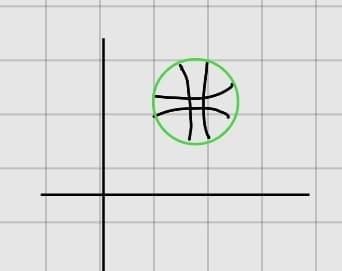
\includegraphics[width=\linewidth]{assets/esfera.jpg}
        \centering
        \label{fig:esfera}
    \end{minipage}
\end{center}
\subsection*{Bola Abierta}
Misma idea que Disco Abierto pero en $\float^{3}$
\[\{(x, y, z) \in \float^{3}: \sqrt[]{(x - a_{0})^{2} + (y - b_{0})^{2} + (z_{0} - c_{0})^{2} < r}\}\] 
\subsection*{Definición formal de Bola Abierta}
\[ Br(P) = \{X = (x_{1}, ..., x_{n}) \in \float^{n} : ||X-P|| < r\}\]
\begin{center}
    \begin{minipage}[b]{0.3\textwidth}
        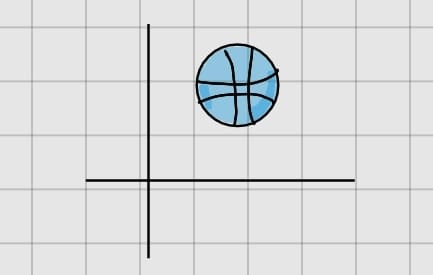
\includegraphics[width=\linewidth]{assets/bola_abierta.jpg}
        \centering
        \label{fig:bola_abierta}
    \end{minipage}
\end{center}
\subsection*{Bola Cerrada}
Misma idea que Disco Cerrado pero en $\float^{3}$
\[\{(x, y, z) \in \float^{3}: \sqrt[]{(x - a_{0})^{2} + (y - b_{0})^{2} + (z_{0} - c_{0})^{2} \ \textcolor{purple}{\le} \ r}\}\]
\textbf{Nota}: Véase $\hyperref[subsec:completar_cuadrados_esfera]{\underline{anexo}}$ para ver ejercicios de completar cuadrados y encontrar el centro y radio de una esfera.
\subsection*{Definición formal de Bola Cerrada}
\[ Br(P) = \{X = (x_{1}, ..., x_{n}) \in \float^{n} : ||X-P|| \le r\}\]
\begin{center}
    \begin{minipage}[b]{0.3\textwidth}
        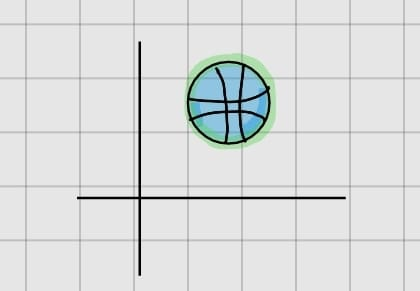
\includegraphics[width=\linewidth]{assets/bola_cerrada.jpg}
        \centering
        \label{fig:bola_cerrada}
    \end{minipage}
\end{center}
\section*{Aclaración sobre enunciados}
Importante siempre prestar atención a la dimensión donde trabajamos. \\
Es decir $x^{2} + y^{2} = 4$ puede representar dos cosas diferentes si estamos en $\float^{2}$ o en $\float^{3}$
\section*{Vectores}
Los vectores tienen dirección, sentido y longitud. \\
Sean dos puntos $P, Q \in \float^{n}$, definimos un vector $V \in \float^{n}$ como $ \bar{PQ} = Q - P$.
\subsection*{Vectores Equivalentes}
Dos vectores son equivalentes si tienen misma dirección, sentido y longitud. 
\subsection*{Vectores Iguales}
Dos vectores son iguales si son equivalentes y además parten del mismo punto.
\subsection*{Suma de Vectores}
Sean $ u, v $ vectores $\in \float^{n}$. La suma de ambos se realiza coordenada a coordenada.
$ u + v = (u_{1} + v_{1}, u_{2} + v_{2}, ..., u_{n} + v_{n})$
\subsection*{Producto por Escalar}
Sea $t \in \float$ y u un vector.
$ t * u = (tu_{1}, tu_{2}, ..., tu_{3})$
\subsection*{Regla del Paralelogramo}
Se utiliza para ver como queda la traslación del vector $u+v$ luego de sumar ambos vectores.
\subsection*{Propiedades de los vectores}
\begin{itemize}
    \item La suma es conmutativa: u + v = v + u
    \item Sea un valor $ t \in \float $, definimos la distributiva con vectores como t(u+v) = tu + tv
\end{itemize}
\subsection*{Norma de un Vector}
Definimos la norma de un vector como $ || V || = \sqrt[]{(v_{1})^{2} + (v_{2})^2 + ... + (v_{n})^2}$ 
\subsection*{Relación entre distancia entre dos puntos y la norma}
Es fácil notar que $ ||B-A|| = ||A-B||. $ 
Definimos la \textbf{equivalencia} de las siguientes fórmulas: 
\[ dist(A, B) = ||B-A|| \equiv ||A-B|| \]
\subsection*{Propiedades de la norma}
\begin{itemize}
    \item $||V||  \ge  0$
    \item $|V| = \sqrt[]{V^{2}}$
    \item $||V|| = dist(V, 0)$
    \item $\alpha \in \float, ||\alpha * V|| = ||\alpha|| * ||V||$: en criollo quiere decir que si multiplico un escalar dentro de la norma, es lo mismo que sacarlo hacia afuera y hacerlo por separado. 
    \item $||V+W|| \le ||V|| + ||W||$: desigualdad Triangular (DT)
    \item $||V-W|| \le ||V|| + ||-W||$: esto tiene sentido pues $||-w||$ es positivo. Entonces queda $||V-W|| \le ||V|| + ||W||$
    \begin{itemize}
        \item Importante: Esto se utiliza mucho para acotar. $ ||V+W||$ y $||V-W||$ se acotan por $ ||V|| + ||-W|$
    \end{itemize}
\end{itemize}
\textbf{Importante}: Si aplico la NORMA a un número, es como aplicar el módulo.
\section*{Producto Interno (Producto Escalar / Producto Punto)}
Sean $u, v \in \float^{n}$. Definimos el producto interno, como la multiplicación \textbf{coordenada a coordenada} de los vectores. \textbf{Siempre devuelve un número.} \\
Hay dos formas de notarlo
\[<u,v> = u * v\]
\subsection*{Vectores Perpendiculares}
Sean $u, v \in \float^{n}$. Si el producto escalar entre dos vectores es 0, entonces los vectores son perpendiculares.
\subsection*{Propiedades del Producto Interno}
\begin{itemize}
    \item $u * u = ||u||^{2}$
    \item Conmutatividad: $u * v = v * u$
    \item Distributividad: Sean $u, v, w \in \float^{n}$, entonces $(u+v) * w = uw + vw$ 
    \item $ t \in \float, (t * u) * v = t * (u * v) = u * (t * v)$
\end{itemize}
\textbf{Importante}: No se pueden multiplicar 3 vectores con el producto interno, porque el producto interno devuelve un NÚMERO. Si multiplico 3 vectores, sería multiplicar primero dos (devuelve un número) y según si es $ > 1 $ o no, estaríamos dilatando/contrayendo otro vector. 
\subsection*{Propiedad importante de la norma y el Producto Interno}
Sean $v, w \in \float^{n}$
\[ v * w = ||v|| * ||w| * cos(\theta)\] con $ 0 \le \theta \le \pi $
\subsection*{Teorema de Cauchy-Schwartz}
$\forall u, v \in \float^{n}$ vale $ |u * v| \le ||u|| * ||v||$ \\
\textbf{Importante}: Si $|u * v| = ||u|| * ||v||$ entonces $ v // u$ (v es paralelo a u)
\section*{Proyecciones}
Sean $v, w \in \float^{n}$. Queremos calcular la proyección de w en la dirección de v. 
\[P_{v}(w) = w * \frac{v}{||w||} * \frac{v}{||v||} = w * v * \frac{v}{||v||^{2}} = \frac{w * v}{v * v} = \frac{w * v}{v^{2}} * v\]
\section*{Producto Vectorial / Cruz (Solo en $\float^{3}$)}
Sean $v, w \in \float^{3}$. Se utiliza para calcular un \textbf{vector perpendicular} a los dos que se nos envían.
\[
\begin{pmatrix}
\hat{i} & \hat{j} & \hat{k} \\
a & b & c\\
d & e & f
\end{pmatrix}
\]
Entonces, el cálculo que hay que hacer es: ((b * f) - (c * e), \textcolor{red}{-} ((a * f) - (c * d)), ((a * e) - (b * d))) \\
\textbf{Importante}: Si este cálculo da 0, entonces los vectores son paralelos.
\subsection*{Propiedades del Producto Vectorial}
\begin{itemize}
    \item (V x W) es perpendicular a V y W.
    \begin{itemize}
        \item Esto es re útil para cuando encontramos una normal para el plano y queremos ver si efectivamente es perpendicular a ambos vectores.
    \end{itemize}
    \item (W x V) = - (V x W): Es decir, no son iguales si los invertimos, si lo invierto le cambio el signo. 
\end{itemize}
\section*{Planos en $\float^{3}$}
Dado un \textbf{vector normal N} y un \textbf{punto de paso P} construimos la ecuación del plano $\pi$ que es perpendicular al \textbf{vector normal} y contiene al punto P (es decir, P verifica la ecuación del plano).
Véase \textbf{\hyperref[subsec:ejercicios_planos]{\underline{anexo}}} para ejercicios de Planos.
\subsection*{Hallar vector normal N de un Plano}
El vector normal N de un Plano lo podemos hallar comúmnente de las siguientres maneras 
\begin{itemize}
    \item Si tenemos 3 puntos, ABC podemos hacer la diferencia y generar 2 vectores directores. Es decir, AB y BC o AB y AC. Luego aplicamos el producto cruz y ya tenemos la normal al plano. Por último podemos tomar cualquier punto.
    \begin{itemize}
        \item Como tenemos la NORMAL tenemos (a, b, c) nos falta d. Para generar d podemos evaluar ax + by + cz con cualquier punto de paso. El número que da como resultado es d.
    \end{itemize}
\end{itemize}
\subsection*{Ecuación Paramétrica del Plano}
$ \pi: \lambda(x_{1}, x_{2}, x_{3}) + \gamma(y_{1}, y_{2}, y_{3}) + (p_{1}, p_{2}, p_{3})$
\subsection*{Ecuación Implícita del Plano}
$ \pi: ax + by + cz = d$
\subsection*{Saber si un punto está en un plano}
Debe verificar la ecuación implícita.
\section*{Rectas Paramétricas}
En $\float^{2} = L:(x,y) = \alpha (v_{1}, v_{2}) + (P_{1}, P_{2}), \alpha \in \float$ \\
En $\float^{3} = L:(x,y,z) = \alpha (v_{1}, v_{2}, v_{3}) + (P_{1}, P_{2}, P_{3}), \alpha \in \float$ \\
Véase \hyperref[subsec:ejercicios_rectas_planos]{\underline{anexo}} para ver ejercicios con rectas y planos.
\subsection*{Rectas Paralelas}
Dos rectas son paralelas sí sus vectores son uno múltiplo del otro.
\subsection*{Rectas Perpendiculares}
Dos rectas son perpendiculares si el producto escalar entre ambos vectores directores da 0.
\subsection*{Rectas Alabeadas}
Dos rectas son alabeadas si no existe intersección entre ellas, y además son paralelas.
\subsection*{Intersección entre dos rectas}
Sean $L_{1}, L_{2}$ dos rectas.
La intersección entre dos rectas se da en un punto específico. Por lo tanto, se espera que la intersección sea un número y además, este número pertenece a $L_{1}$ Y $L_{2}$
\subsection*{Casos de Rectas y Planos}
\begin{itemize}
    \item Si tengo plano + 2 rectas: Si se cruzan o son paralelas, entonces existe un único plano.
    \item Si tengo plano + 1 recta: Existen infinitos planos que la contenga.
\end{itemize}
\section*{Curvas}
Son un conjunto de puntos por los que pasó una partícula dada a lo largo del tiempo.
La trayectoria, el movimiento que hace en cada tiempo t la partícula va dejando una marca y forma una curva. \\
Las funciones son de la forma 
\[
f(t) =
\begin{cases} 
x = x(t) \\
y = y(t)
\end{cases}
\]
\textbf{Nota}: En general, una curva en $\float^{n}$ es la imagen de una función $ \alpha(t)$ continua de $\float$ en $\float^{n}$. Es decir, $Im \ \alpha = C$ \\
\textbf{Ej.}: Una recta en $\float^{2}$ es la imagen de una curva paramétrica. \\
Véase \hyperref[subsec:curvas_ejemplo]{anexo} para ver como parametrizar.
\subsection*{Criterio de la Recta Vertical}
No todas las curvas representan funciones. Para poder ver esto de una forma fácil, recordemos qué es una función. Una función es una máquina que espera un valor y da otro. \\
Ahora, es importante que para diferentes valores tienen que dar diferentes resultados. \\
Si existen valores que dan el mismo resultado, entonces no es una función. 
\begin{center}
    \begin{minipage}[b]{0.3\textwidth}
        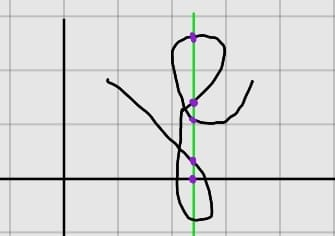
\includegraphics[width=\linewidth]{assets/criterio_recta_vertical.jpg}
        \centering
        \label{fig:criterio_recta_vertical}
    \end{minipage}
\end{center}
\textbf{Importante}: Todos los gráficos son curvas pero no toda curva es gráfico de función.
\subsection*{Paramétrización de la Curva}
Existen infinitas parametrizaciones para una misma curva. Esto quiere decir, que una misma partícula puede realizar una trayectoria de mil maneras diferentes. \\
Denotamos la parametrización de una curva como: $C = \{(x(t), y(t)) \ / \ t \in \float \}$ y decimos que es paramétrica porque espera un \textbf{solo} parámetro. \\
Las parametrizaciones nos dan descripciones dinámicas mientras que las que no tienen un parámetro t son estáticas.
\subsection*{¿Qué no nos dice la ecuación implícita de una curva?}
Las ecuaciones en x y y describe \textbf{donde} ha estado la partícula pero no nos dice \textbf{cuándo} ha estado la partícula en un punto en particular. 
\subsection*{¿Qué nos dice la ecuación paramétrica de una curva?}
La ventaja es que nos dicen \textbf{cuándo (t)} estuvo la partícula en un punto (x, y) y la dirección en su trayectoria.
\subsection*{Ejemplo de Curvas}
Recordemos que básicamente una curva se arma gracias a la trayectoria de una partícula que hace cierto movimiento a lo largo del tiempo. \\
Este tiempo se llama t, y podemos ir viendo el movimiento de la partícula gracias a la ecuación paramétrica. A medida que t aumenta, esa es la dirección que toma la partícula. \\
\[
f(t) =
\begin{cases} 
x = t^{2} - 2t \\
y = t - 1
\end{cases}
\]
Si nos ponemos a darle valores a t, vamos a ir obteniendo valores de x e y, que básicamente los podemos graficar en un plano.
\[\begin{minipage}[b]{0.7\textwidth}
    \includegraphics[width=\linewidth]{assets/curva.png}
\end{minipage}\]
Parece entonces en este ejemplo, que la partícula hizo la trayectoria de una parábola. Busquemos entonces la ecuación implícita para ver qué curva representan las ecuaciones paramétricas.
\[
f(t) =
\begin{cases} 
x = t^{2} - 2t \\
y = t - 1 \equiv y+1 = t
\end{cases}
\]
Entonces, $ x = (y+1)^{2} - 2(y+1) \equiv x = y^{2} -4y +3$ \\
Efectivamente podemos notar que la partícula, gracias a esas ecuaciones parámetricas y dando el tiempo t fuimos formando la curva paramétrica (parábola) $ x = y^{2} -4y +3$. \\
Entonces ¿cuál es la diferencia entre tener la ecuación paramétrica con un parámetro t o tener la que depende de x e y? La diferencia es que con la parámetrica podemos saber en qué lugar estaba la partícula en un tiempo t. \\
\subsection*{Restringiendo los posibles valores t de la Curva}
Se utilizan intervalos. Es decir, nosotros podemos decir qué trayectoria recorre la partícula, desde qué t hasta qué t. \\
Esto se define como $ x = f(t) \ y \ y = g(t) \ a \le t \le b$ donde el \textbf{punto inicial} es (f(a), g(a)) y el \textbf{punto final} es (f(b), g(b)). \\
Ejemplo: $ x = (t^{2} - 2t) \ y = (t+1) \ 0 \le t \le 4$
\[\begin{minipage}[b]{0.5\textwidth}
    \includegraphics[width=\linewidth]{assets/curva_delimitada.png}
\end{minipage}\]
\subsection*{Circunferencias Paramétricas}
Se suelen representar con coseno y seno.
\[x = cos(t), y = sen(t), 0\le t < 2\pi\]
Si damos unos valores t y dibujamos en el plano, veremos que está realizando una circunferencia de radio 1.
\[\begin{minipage}[b]{0.5\textwidth}
    \includegraphics[width=\linewidth]{assets/cost_sent.png}
\end{minipage}\]
Observamos que $x^{2} + y^{2} = cos^{2}\ t + sen^{2}\ t = 1$. En este caso la circunferencia se va completando gracias a la trayectoria del punto que va en sentido antihorario. \\
\[x = sen(2t), y = cos(2t), 0\le t < 2\pi\]
Este es parecido al anterior, la diferencia es que ahora vamos al \textbf{doble de velocidad}. Antes con cos(t) y sen(t) ibamos de 0 a 2pi \textbf{una vez}. Acá, al estar multiplicado el t por 2, lo que va a hacer es que vamos a recorrer en 2pi \textbf{dos veces} la circunferencia (cada $\pi$ recorrimos la circunferencia entera). Pero ojo, esta es sen(2t) y cos(2t) entonces, está invertido el recorrido. Acá se hace en sentido horario.
\[\begin{minipage}[b]{0.7\textwidth}
    \includegraphics[width=\linewidth]{assets/sen2t_cos2t.png}
\end{minipage}\]
Nótese que llegamos a 3.14 y ya recorrió toda la circunferencia gracias al 2t (antes recorría la mitad). Sin embargo, el deslizador indica que le falta todavía una vuelta para dar. \\
\textbf{Conclusión}: Podemos ver que dos parametrizaciones diferentes, representan la misma curva (circunferencia), pero recorrida a diferente velocidad.
\subsection*{Deslizadores en GeoGebra}
Nos permiten simular como una partícula se mueve realizando la curva. \\
\[\begin{minipage}[b]{0.9\textwidth}
    \includegraphics[width=\linewidth]{assets/geogebra.png}
\end{minipage}\]
Por si requiere orientación, observe este \href{https://www.youtube.com/watch?v=Sb1W73Vb_98&list=PLvwXmp0qN7l2Fg-D4eWt57Fri_fYN-Sw5&index=2&t=671s}{vídeo}.
\[\begin{minipage}[b]{0.9\textwidth}
    \includegraphics[width=\linewidth]{assets/resultado_geogebra_curva.png}
\end{minipage}\]
\section*{Coordenadas Cartesianas y Polares}
\subsection*{Coordenada Cartesiana}
Permite representar un punto en el plano mediante un par ordenado de números llamados coordenadas. \\
Ej.: $P = (1, 2)$ está dado de forma cartesiana.
\subsection*{Coordenada Polar}
Permite representar un punto P mediante el par ordenado $(r, \theta)$ y r, $\theta$ se llaman coordenadas polares de P. \\
\textbf{Recordatorio}: r: largo, $\theta$: ángulo desde el (0, 0)
\[\begin{minipage}[b]{0.3\textwidth}
    \includegraphics[width=\linewidth]{assets/coordenadas_polares.png}
\end{minipage}\]
\textbf{Nota}: Si $r>0$ el punto $(r, \theta)$ está en el mismo cuadrante que $\theta$. Si $r<0$ está en el cuadrante opuesto del polo $(-r, \theta) \equiv (r, \theta + \pi)$
\[\begin{minipage}[b]{0.3\textwidth}
    \includegraphics[width=\linewidth]{assets/coordenadas_polares_2.png}
\end{minipage}\]
\textbf{Importante}: $\theta$ se mide en radianes y normalmente el rango es $0 \le \theta < 2\pi$ pues el 0 es lo mismo que incluir el $2\pi$
\subsection*{Coordenadas Polares a Cartesianas}
La fórmula se deduce a partir de lo siguiente $ cos \ (\theta) \ = \ \frac{x}{r} \ , \ sen(\theta) = \frac{y}{r}$
\[\begin{minipage}[b]{0.3\textwidth}
    \includegraphics[width=\linewidth]{assets/coordenadas_polares_a_cartesiana.png}
\end{minipage}\]
Masajeando un poco, nos queda
\[x = r * cos(\theta), \ y = r * sen(\theta)\]
\subsection*{Coordenadas Cartesianas a Polares}
Podemos calcularlo a partir del pasaje o la figura anterior. Por lo tanto nos quedaría 
\[r^{2} = x^{2} + y^{2},\ tan(\theta) = \frac{y}{x} \]
Véase \hyperref[subsec:pasaje_coord_polares_cartesianas]{anexo} para ejercicios acerca de los pasajes en este tema. 
\section*{Curvas Polares}
La gráfica de una ecuación polar $r = f(\theta)$ o de manera más general $F(r, \theta) = 0$ consiste de todos los puntos P que tienen al menos una representación polar $(r, \theta)$. \\
\textbf{Ej.}: $ r = 2 $ representa a $F(2, \theta)$ y esto sería básicamente una circunferencia con centro 0 y de radio 2. ¿Por qué una circunferencia? Porque $\theta$ es un ángulo, y los ángulos van desde $0\le \theta < 2\pi$
\[\begin{minipage}[b]{0.9\textwidth}
    \includegraphics[width=\linewidth]{assets/curvas_polares_graficos.png}
\end{minipage}\]
En la imagen anterior podemos ver varias curvas polares que representan circunferencias con centro 0. \\

\textbf{Ej.}: $ \theta = 1$ representa a una curva que posee siempre el ángulo $\theta = 1 \ (medido \ en \ radianes)$ sin ninguna restricción acerca de p. 
\[\begin{minipage}[b]{0.6\textwidth}
    \includegraphics[width=\linewidth]{assets/curva_polar_solo_angulo.png}
\end{minipage}\]
\subsection*{Pasaje de Curva dada en forma Polar a Curva dada en Ecuación Cartesiana}
\[\begin{minipage}[b]{0.7\textwidth}
    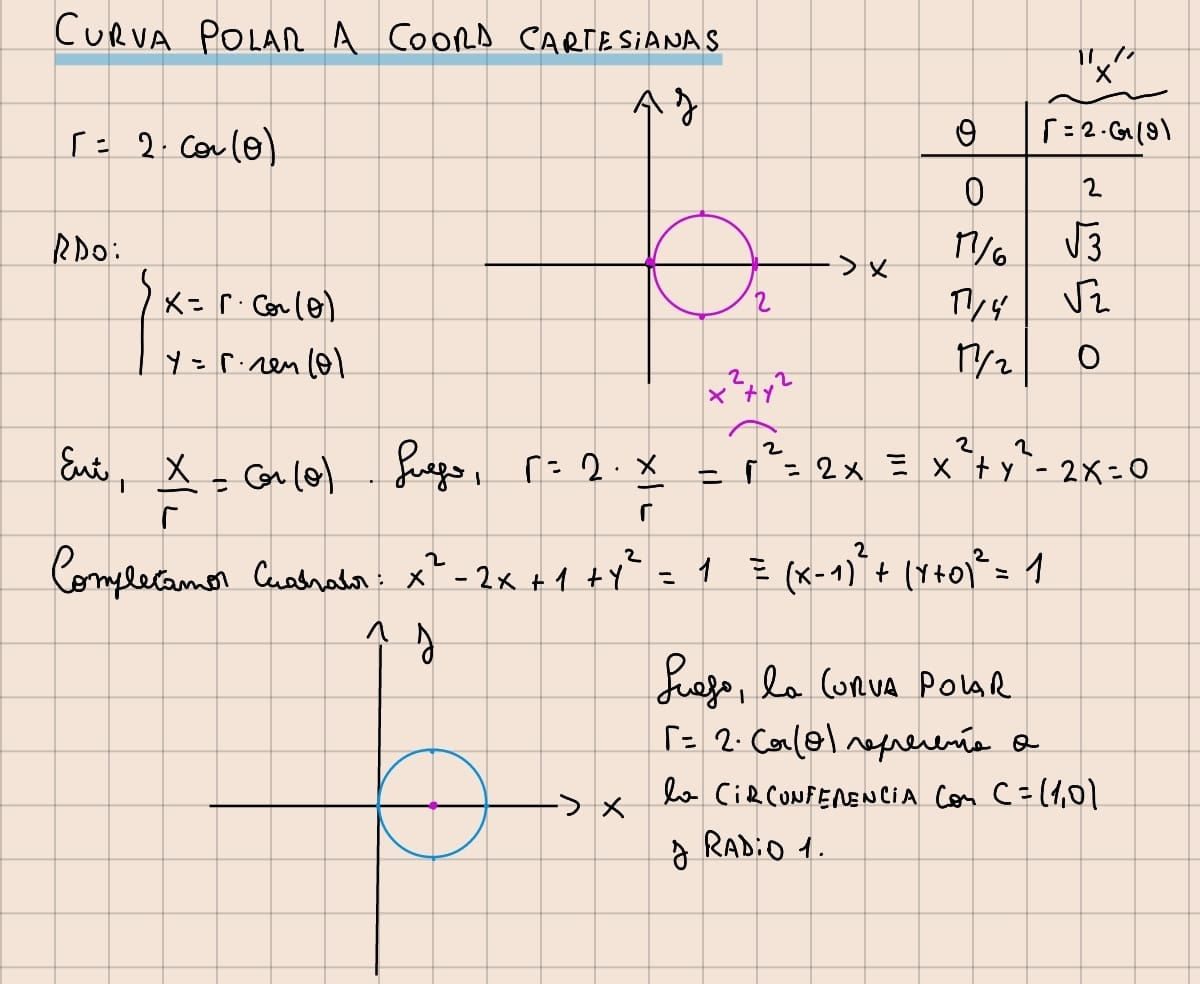
\includegraphics[width=\linewidth]{assets/curva_polar_a_coord_cartesianas.jpg}
\end{minipage}\]
\textbf{Importante}: Véase que despejamos $x = r * cos(\theta)$ para ver qué vale $cos(\theta)$ porque nuestro ejercicio tenia un $2 * cos(\theta)$. Nos queda más fácil para aplicar $r^{2} \equiv x^{2} + y^{2}$
\subsection*{Cardioide}
\[\begin{minipage}[b]{0.5\textwidth}
    \includegraphics[width=\linewidth]{assets/cardioide.png}
\end{minipage}\]
\subsection*{Rosa de 4 Pétalos}
\[\begin{minipage}[b]{0.6\textwidth}
    \includegraphics[width=\linewidth]{assets/rosa_4_petalos.png}
\end{minipage}\]
\textbf{Preguntar}: ¿Por qué $ r = 2 * cos(\theta)$ es fácil pasarlo a ecuación cartesiana y no pasa lo mismo con $ r = 1 + sen(\theta) $ o $ r = cos(2 \theta)$?
\section*{Cónicas}
Se llaman cónicas porque resultan de cortar un cono con un plano. 
\subsection*{Parábolas}
Una parábola es el conjunto de puntos en el plano que estan a igual distancia de un punto fijo F (llamado \textbf{foco}) y una recta fija (llamada \textbf{directriz}). \\
El punto entre el foco y la directriz se llama \textbf{vértice}. \\
La recta perpendicular a la directriz que pasa por el foco se llama \textbf{eje} de la parábola.
\[\begin{minipage}[b]{0.4\textwidth}
    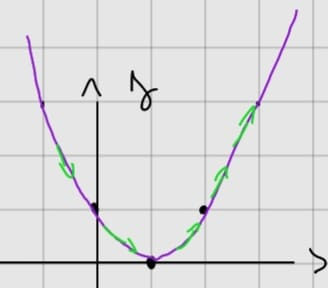
\includegraphics[width=\linewidth]{assets/parabola.png}
\end{minipage}\]
\subsection*{Relación entre el Foco y la Directriz}
Si el foco está en el punto $(0, p)$ entonces la directriz tiene la ecuación $y = -p$. 
Esto quiere decir que la \textbf{distancia del foco al vértice} es la \textbf{misma} que la \textbf{distancia de la directriz al vértice.}
\subsection*{Distancia de un punto $P(x, y)$ de la parábola al Foco y Directriz}
\textbf{P a Foco}: $|PF| = \sqrt[]{x^{2} + (y-p)^{2}}$ \\
\textbf{P a Directriz}: $ |y+p| = \sqrt[]{x^{2} + (y-p)^{2}} $ \\
La ecuación equivalente que se consigue desarrollando $ |y+p| = \sqrt[]{x^{2} + (y-p)^{2}} $ es $x^{2} = 4py \equiv \frac{1}{4p} x^{2} = y \equiv ax^{2} = y  $
\subsection*{Parametrizando una Función}
Consideremos $ax^{2} = y$, la manera de parametrizarla es de la siguiente forma 
\[
f(t) =
\begin{cases} 
x = t \\
y = at^{2}
\end{cases}
\]
\subsection*{Efecto del Foco y la Directriz con la Parábola}
Más cerca esté de origen el punto P, entonces más chica será la distancia entre el foco y la directriz y la parábola será menos ancha. 
\[\begin{minipage}[b]{0.6\textwidth}
    \includegraphics[width=\linewidth]{assets/parabola_1.png}
\end{minipage}\]
\[\begin{minipage}[b]{0.6\textwidth}
    \includegraphics[width=\linewidth]{assets/parabola_2.png}
\end{minipage}\]
\subsection*{¿Hacia donde abre la parábola?}
\begin{itemize}
    \item $x^{2} = 4py$ (directriz en y, foco (0, p))
    \begin{itemize}
        \item $p > 0$: Hacia arriba
        \item $p < 0$: Hacia abajo
    \end{itemize}
    \item $y^{2} = 4px$ (directriz en x, foco (p, 0))
    \begin{itemize}
        \item $p>0$: Hacia la derecha
        \item $p<0$: Hacia la izquierda
    \end{itemize}
\end{itemize}
\textbf{Recordatorio}: La directriz y el foco están en el eje contrario al que tiene el cuadrado.
\subsection*{Elipses}
Una elipse es el conjunto de planos en un plano cuya suma de sus distancias a dos puntos $F_{1}$ y $F_{2}$ es una constante. Estos dos puntos fijos se llaman \textbf{focos}. 
\subsection*{Cálculo de los focos}
La fórmula es: $c^{2} = a^{2} - b^{2}$
\subsection*{Formas de armar una Elipse}
Existe un concepto que es eje mayor y eje menor. Encontrando el eje mayor ya sabemos donde están posicionados los focos y los vértices. \\
$\frac{x^{2}}{a^{2}} + \frac{y^{2}}{b^{2}} = 1 \ con \ a \ge b > 0$: tiene focos $(\pm c, 0)$ donde $c^{2} = a^{2} - b^{2}$ y vértices $(\pm a, 0)$ \\
$\frac{x^{2}}{b^{2}} + \frac{y^{2}}{a^{2}} = 1 \ con \ a \ge b > 0$: tiene focos $(0,  \pm c)$ donde $c^{2} = a^{2} - b^{2}$ y vértices $(0, \pm a)$ \\
\textbf{En criollo}: La letra que tiene un denominador más grande, es el que tiene los focos y el vértice (eje mayor). El eje mayor sería hacia donde es más grande. El número más grande siempre es \textbf{a}. \\
\textbf{Tips}: Siempre recordar que si me dan un foco ya puedo determinar el eje mayor; mismo con si me dan un vértice. Recordar también que el vértice depende de \textbf{a} esto quiere decir es que si me dan el vértice me dieron el eje mayor. \\
En la teoría no hay más que eso, véase \hyperref[subsec:elipses_ejercicios]{anexo} para ver ejercicios de elipses. \\
\subsection*{Hipérbolas}
Una Hipérbola es el conjunto de todos los puntos en un plano cuya diferencia de sus distancias a dos puntos fijos $F_{1}$ y $F_{2}$ (los focos) es una constante. 
\subsection*{Cálculo de los focos}
La fórmula es: $c^{2} = a^{2} + b^{2}$
\subsection*{Formas de armar una Hipérbola}
Existe un concepto que es eje mayor y eje menor. Encontrando el eje mayor ya sabemos donde están posicionados los focos y los vértices. \\
$\frac{x^{2}}{a^{2}} - \frac{y^{2}}{b^{2}} = 1$: tiene focos $(\pm c, 0)$ donde $c^{2} = a^{2} + b^{2}$, vértices $(\pm a, 0)$ y asíntotas $y = \pm \frac{b}{a}x$ \\
$\frac{y^{2}}{a^{2}} - \frac{x^{2}}{b^{2}} = 1$: tiene focos $(0,  \pm c)$ donde $c^{2} = a^{2} + b^{2}$, vértices $(0, \pm a)$ y asíntotas $y = \pm \frac{a}{b}x$ \\
En la teoría no hay más que eso, véase \hyperref[subsec:hiperbolas_ejercicios]{anexo} para ver ejercicios de elipses. 
\section*{Cónicas Desplazadas}
Son exactamente las mismas maneras, solo que acá en vez de x e y es (x-k) y (y-k).
Entonces, ej hipérbola con eje mayor x
\begin{itemize}
    \item $vertices = (centroX \pm a, centroY)$
    \item $focos = (centroX \pm c, centroY)$
    \item $hiperbolas = -\frac{b}{a}(x - centroX) \ y \ \frac{b}{a}(x - centroX) $
\end{itemize}
\section*{Parametrización de Cónicas}
Un problema muy común es que nos den ciertas cónicas para parametrizar. Normalmente se nos pide una circunferencia pero está bueno tener en cuenta las demás. \\
\textbf{Nota}: Cuando hablemos de partidas con cos y sen, a cual aplicar cos y a cual sen es según la regla de la mano derecha. 
\subsection*{Parábola}
Una de las mas sencillas, la idea es poner todo el cálculo en y. \\
Ej.: $x = y^{2} + 4$
\[
\begin{cases} 
x = t \\
y = t^{2} + 4
\end{cases}
\]
\subsection*{Circunferencia}
\[
\begin{cases} 
x = r * cos(t) + cx \\
y = r * sin(t) + cy
\end{cases}
\]
donde: 
\begin{itemize}
    \item r: Radio
    \item c: Centro, y por lo tanto, cx es la coordenada x del centro, análogamente con y.
    \item t: Parámetro, normalmente va a ser entre $[0, 2\pi)$
\end{itemize}
\textbf{Ojo}: Recordar que el radio debe sacarse la raíz cuadrada, porque normalmente cuando tenemos la fórmula corresponde a $r^{2}$ \\
Ej.: $x^{2} + (y-3)^{2} = 9$ corresponde a 
\[
\begin{cases} 
x = 3 * cos(t) + 0 \\
y = 3 * sin(t) + 3
\end{cases}
\]
\subsection*{Elipse}
\[
\begin{cases} 
x = a * cos(t) + cx \\
y = b * sin(t) + cy
\end{cases}
\]
donde: 
\begin{itemize}
    \item a: Semieje Mayor 
    \item b: Semieje Menor 
    \item c: Centro, y por lo tanto, cx es la coordenada x del centro, análogamente con y.
    \item t: Parámetro, normalmente va a ser entre $[0, 2\pi)$
\end{itemize}
\textbf{Ojo}: Recordar que en las elipses, el denominador está elevado al cuadrado. Por lo tanto, considerarlo con la raíz cuadrado.
\subsubsection{Truco}
Muchas veces se nos dan las elipses/hipérbolas de esta forma $9z^{2} + x^{2} = 1$ \\
¿Cual es el problema acá? que una elipse tiene denominador. \\
¿Cómo pasamos el 9 al denominador? Fácil: $\frac{z^{2}}{\frac{1}{9}}$ \\
Entonces ¿quién es a? en este caso, $\frac{1}{3}$. 
\subsection*{Hipérbolas}
Análogo a Elipse, pero la diferencia es que la variable que depende del cos está negada. 
\[
\begin{cases} 
x = -a * cos(t) + cx \\
y = b * sin(t) + cy
\end{cases}
\]
\section*{Superficies Cuadráticas ($\float^{3}$)}
En cualquier lado tenemos 2 direcciones para movernos libres. Podemos movernos dentro de la curva, o por las rectas. \\
$ax^{b} + by^{2} + cz^{2} + dxy + eyz + fxz + gx + hy + iz + j = 0$ \\
No es necesario recordar la fórmula, lo que si está bueno saber que mediante rotaciones y traslaciones esta ecuación podemos reescribirlo de diferentes maneras. 
\begin{itemize}
    \item Tipo 1: $ax^{2} + by^{2} + cz^{2} + j = 0$
    \item Tipo 2: $ax^{2} + by^{2} + iz = 0$
\end{itemize}
Estas diferentes maneras de verlo nos genera todas las cuadricas que necesitamos. \\
Ej.: $x^{2} + \frac{y^{2}}{4} + z^{2} = 1$. Este es un caso particular del primer tipo que escribimos arriba. \\
Para ver la resolución, véase \hyperref[subsec:trazas_superficies]{\underline{anexo}} \\
\textbf{Importante}: Lo más importante de todas estas cosas es saber reconocer las cuádricas a ojo y saber cortarlas con distintos planos. No es necesario saber graficarlas pero sí tener una idea de como son. \\
Si quiere observar la tabla de cúadricas, véase \hyperref[subsec:tabla_cuadricas]{\underline{anexo}}
\subsection*{Variables Dependientes $\&$ Variables Independientes}
En contextos de $\float^{3}$ decimos que una variable es independiente si tiene un grado mayor que la otra. \\
Ej. $y = z^{2}$ nos indica que $z^{2}$ es la variable independiente mientras que \textbf{y} es la variable dependiente. Esta relación claramente nos indica que $y \ge 0 $ siempre.
\subsection*{Curvas de Nivel}
Una curva de nivel $f(x,y) = k$ es el conjunto de todos los puntos en el dominio de $f$ en el cual $f$ toma un valor dado k. En palabras más simples, señala donde tiene una altura k la gráfica de f. \\

\subsection*{Trazas}
En un conjunto tridimensional es muy dificil de observar. \\
Las trazas nos ayudan a través de planos paralelos a los ejes coordenados cortar una superficie.
\begin{itemize}
    \item z = k es un plano paralelo al plano xy
    \item y = k es un plano paralelo al plano xz
    \item x = k es un plano paralelo al plano yz
\end{itemize}
Cuando yo hago un corte a una superficie con una traza, me queda una curva. Si miro como van siendo esas curvas a medida que las corto con distintas trazas esto me da una idea de como va a ser esa superficie. \\
\textbf{Importante}: Muchas veces algunas superficies pueden ser parecidas si hacemos pocas trazas. Por lo tanto la idea \textbf{siempre} es hacer trazas que marquen la diferencia. \\
Para ver ejemplos sobre lo que acabo de marcar como importante, véase \hyperref[subsec:dibujando_cuadricas_con_trazas]{\textbf{\underline{anexo ejemplos 1 y 3}}} 
\subsection*{Dibujando Cuádricas con Trazas}
\label{subsec:dibujando_cuadricas_con_trazas}
1. $z^{2} = x^{2} + y^{2}$ \\
\textbf{Nota}: Recuerde observar siempre bien los enunciados. En este caso podemos darnos cuenta que siempre z será positivo.
\begin{itemize}
    \item Interseco / Corto con traza z = cte.
    \begin{itemize}
        \item $ z = 0 \implies x^{2} + y^{2} = 0 \iff x = y = 0$
        \item $ z = 1 \implies x^{2} + y^{2} = 1$
        \item $ z = -1 \implies x^{2} + y^{2} = 1$
        \item $ z = 2 \implies x^{2} + y^{2} = 4$
        \item $ z = -2 \implies x^{2} + y^{2} = 4$
    \end{itemize}
    \item Interseco / Corto con traza x = cte
    \begin{itemize}
        \item $x = 0, \ z^{2} = y^{2} \iff \longitud{z} = \longitud{y} \implies z = \longitud{y} \ y \ z = -\longitud{y}$
    \end{itemize}
\end{itemize}
Esta cuádrica es el cono. \\
2. $z = \sqrt[]{x^{2} + y^{2}}$ \\
Lo primero que notamos es que $z$ es una variable dependiente y está ligada a lo que valga $x^{2} + y^{2}$. Por lo tanto, como ambos términos son positivos, entonces $z \ge 0 $. \\
De esta observación descartamos trazas con $ z = -k $ \\
3. $z = x^{2} + y^{2}$ \\
Mismo que el ejemplo anterior, notamos que $z \ge 0$ y está ligada. 
\begin{itemize}
    \item Interseco / Corto con traza z = cte.
    \begin{itemize}
        \item $z=0 \implies x^{2} + y^{2} = 0$
        \item $z=1 \implies x^{2} + y^{2} = 1$
    \end{itemize}
\end{itemize}
En este ejemplo particular podemos ver que las \textbf{trazas} nos dieron exactamente igual que en el ejemplo 1. Esto indica que claramente tienen un parecido, pero como son diferentes ecuaciones, algo nos falta. Tomemos más trazas. 
\begin{itemize}
    \item Interseco / Corto con traza x = cte.
    \begin{itemize}
        \item $x=0, \ z=y^{2}$. Es una parábola.
    \end{itemize}
\end{itemize}
Esto es un Paraboloide.
\subsection*{Recta Generatriz}
Es una recta que tomo en $\float^{3}$ que normalmente es para tomar paralelas y generar cortes.
\subsection*{Cilindro}
Es el conjunto de puntos que atraviesan la curva plana $x^{2} + y^{2} = 1$ y que son paralelas a la recta generatriz. \\
Cuando hago un corte, asignando un valor de z nos genera un cilindro.
\[\begin{minipage}[b]{0.6\textwidth}
    \includegraphics[width=\linewidth]{assets/cilindro.png}
\end{minipage}\]
\subsection*{Cilindro Parabólico (generado por una parábola)}
Tomo una recta generatriz en el eje y $x=z=0$.
\[\begin{minipage}[b]{0.5\textwidth}
    \includegraphics[width=\linewidth]{assets/cilindro_parabolico.png}
\end{minipage}\]
\subsection*{Cilindro Hiperbólico (generado por una hipérbola)}
Toma una recta generatriz (eje?)
\[\begin{minipage}[b]{0.5\textwidth}
    \includegraphics[width=\linewidth]{assets/cilindro_hiperbolico.png}
\end{minipage}\]
\section*{Parametrización para Curva dada por intersección de dos superficies}
1. $z = 3x^{2} \ x^{2} + 4y = 1$ 
\begin{itemize}
    \item 1. Recordar es que cuando hablamos de superficies estamos en $\float^{3}$. 
    \item 2. Recordar que como estamos hablando de una curva que se forma en base a una intersección, entonces la curva estará en $\float^{3}$ y requerirá solo de un parámetro.
    \item 3. Hay dos formas de encarar este tipo de ejercicios 
    \begin{itemize}
        \item 1. Si tienen una variable en común, con mismo grado y todo, despejamos todo en base a una variable.
        \item 2. Si no tienen una variable en común, lo que podemos hacer es básicamente hacer reemplazos.
    \end{itemize}
\end{itemize}
En este ejercicio particular, como $z = 3x^{2}$ y $x^{2} + 4y = 1$ tienen en común al $x^{2}$ podemos hacer $z = 3x^{2} \ y = \frac{x^{2} + 1}{4}$
Entonces, para armar la parametrización basta con decir que $ \alpha(x) = (x^{2}, \frac{x^{2} + 1}{4}, 3x^{2})$ con $x \in \float $ \\
2. $x^{2} + y^{2} = 4 \ z = 3$
\begin{itemize}
    \item 1. Recordar que como hablamos de superficies estamos en $\float^{3}$.
    \item 2. Recordar que como estamos hablando de una curva que se forma en base a una intersección, entonces la curva estará en $\float^{3}$ y requerirá solo de un parámetro.
    \item 3. Si observamos detenidamente ambas ecuaciones vemos que no tienen los mismos términos en común.
    \begin{itemize}
        \item Lo que podemos hacer primero es notar que $x^{2} + y^{2} = 4$ es una esfera centrada en el origen con radio 2. 
        \item Como sabemos parametrizar las circunferencias, entonces sabemos que por ahora nuestra parametrización consta de $\alpha(t) = (2 \ cos(t), 2 \ sen(t))$ pero nos falta el último término.
        \item Como z es constante, entonces lo que nos quiere decir es que la circunferencia estará en $z = 3$.
    \end{itemize}
\end{itemize} 
Por lo tanto, la respuesta es $\alpha(t) = (2 \ cos(t), 2 \ sen(t), 3)$ con $t \in [0, 2\pi]$. \\
Esta parametrización indica que es básicamente una esfera que vive en $z=3$ \\
\textbf{Nota}: Da exactamente igual si colocamos $\pi$ incluido o no. Si lo incluimos entonces no será inyectiva, pero en nuestras aplicaciones prácticas no afecta en nada. \\
\textbf{Importante}: ¿Qué hubiese pasado si intentabamos despejar la ecuación de $x^{2} + y^{2} = 4$? Nos queda lo siguiente $ y = \pm \sqrt[]{4-x^{2}}$. Al separarse en dos caminos, no podría ser parte de una parametrización válida. \\
3. $x^{2} + y^{2} = 1 \ x + y + z = 1$
\begin{itemize}
    \item 1. Recordar que como hablamos de superficies estamos en $\float^{3}$.
    \item 2. Recordar que como estamos hablando de una curva que se forma en base a una intersección, entonces la curva estará en $\float^{3}$ y requerirá solo de un parámetro.
    \item 3. Si observamos detenidamente no tienen términos en común. Pero, la primera ecuación no habla de $z$ por lo tanto está libre. 
    \item 4. Lo que podemos hacer en este caso es, como en el ejemplo anterior, como conocemos qué es $x^{2} + y^{2} = 1$. Podemos decir que $\alpha(t) = (cos(t), sen(t), ???)$.
    \item 5. Nos falta calcular z porque estamos en $\float^{3}$ pero sabemos que $z = 1-x-y$. 
    \item 6. Por lo tanto $\alpha(t) = (cos(t), sen(t), 1-x-y) \equiv \alpha(t) = (cos(t), sen(t), 1-cos(t)-sen(t)) $.
\end{itemize}
Por lo tanto, la respuesta es $\alpha(t) = (cos(t), sen(t), 1-cos(t)-sen(t))$ con $t \in [0, 2\pi]$. \\
\textbf{Importante}: Si se quisiera verificar si las parametrizaciones que encontramos son correctas, debería validar ambas ecuaciones.
4. $(x-y)^{2} + z^{2} = 4 \ z = x+y$
\begin{itemize}
    \item 1. Recordar que como hablamos de superficies estamos en $\float^{3}$.
    \item 2. Recordar que como estamos hablando de una curva que se forma en base a una intersección, entonces la curva estará en $\float^{3}$ y requerirá solo de un parámetro.
    \item 3. En este caso podemos observar que los términos de ambas ecuaciones se parecen, podemos comenzar reemplazando a $z^{2}$ por $z=x+y$.
    \item 4. Haciendo esto nos queda $x^{2} + y^{2} = 2$. Entonces nos queda algo que ya súper conocemos. 
\end{itemize}
Por lo tanto, $\alpha(t) = (\sqrt[]{2} \ cos(t), \ \sqrt[]{2} \ sen(t), \sqrt[]{2} \ cos(t) \ + \ \sqrt[]{2} \ sen(t)) $ con $t \in [0, 2\pi]$
\subsection*{Intersección y Parametrización de Parcial}
\[\begin{minipage}[b]{0.9\textwidth}
    \includegraphics[width=\linewidth]{assets/curva_ejercicio_parcial.png}
\end{minipage}\]
Respiremos por un momento, y notemos que en dos lados al mismo tiempo tenemos z. \\
La primera parece una parábola, mientras que la segunda no tenemos certeza porque no sabemos cuanto vale z. \\
La idea, sería meter una ecuación dentro de la otra para empezar a laburar. \\
Por lo tanto $x^{2}+4 = 2x^{2}+3y^{2}$, hasta ahora no sabemos que cónica se armó. \\
Luego $4 = x^{2}+3y^{2}$ y esto es algo que claramente conocemos pero con una forma media rara. \\
Si rearmamos un poco los términos nos queda $4 = x^{2} + \frac{y^{2}}{\frac{1}{3}}$, y luego si dividimos por 4 $\frac{x^{2}}{4} + \frac{y^{2}}{\frac{\frac{1}{3}}{4}} = 1$ y finalmente: $\frac{x^{2}}{4} + \frac{y^{2}}{\frac{4}{3}} = 1$ \\
Por lo tanto, si recordamos la parametrización de la elipse nos quedaría algo así: 
\[
\begin{cases}
    x = 2 * cos(t) \\
    y = \sqrt{\frac{4}{3}} * sen(t) \ con \ t \ \in [0, 2\pi)
\end{cases}
\] 
Ahora por último vemos cuanto vale z en base a los valores anteriormente conocidos $ z = 4 cos(t^{2}) + 4$ \\
Por lo tanto, nuestra parametrización nos quedó de la siguiente forma: $r(t) = (2 * cos(t), \sqrt{\frac{4}{3}} * sen(t), 4 cos^{2}(t) + 4)$ con $t \in [0, 2\pi)$ \\
Si tenemos duda acerca de nuestra parametrización podemos meter coordenada a coordenada en las definiciones y ver si verifica efectivamente ambas ecuaciones. \\
El inciso b nos pide verificar que un punto P = (1, -1, 5) está en la curva C. Como nosotros estamos con una parametrización en base a t, necesitamos encontrar un t que nos dé efectivamente este punto. Por lo tanto, planteamos un sistema
\[
\begin{cases}
    1 = 2 * cos(t) \\
    -1 = \sqrt{\frac{4}{3}} * sen(t) \\
    5 = 4 * cos^{2}(t) + 4
\end{cases}
\] 
\textbf{Importante}: Cuando tenemos el coseno al cuadrado primero hacer el cos sin el cuadrado, y el resultado elevarlo al cuadrado. \\
Lo primero que podemos hacer básicamente despejar una ecuación sencilla. Podemos empezar sabiendo que $\frac{1}{2} = cos(t)$ ahora lo que podemos hacer básicamente es hacer $t = cos'(\frac{1}{2})$ y esto nos arroja $\frac{\pi}{3}$ \\
Entonces ahora, con este t evaluemos en todos los casos y veamos si efectivamente vale. Probando vemos que la segunda no se verifica. \\
Despejando de la segunda, nos queda $\frac{5\pi}{3}$. \\
Ahora sí, si evaluamos en cada una de las coordenadas de r nos queda (1, -1, 5). \\
Por último nos piden hallar la ecuación de la recta tangente a C en el punto P. \\
Lo que vamos a considerar ahora, es como importante el t0 que encontramos, es decir $\frac{5\pi}{3}$ porque hay que evaluar en ese lugar a la derivada. \\
Si derivamos a r nos queda $r'(t) = (-sen(t), \sqrt{\frac{4}{3}} * cos(t), 4 * (2 cos(t) * -sen(x))) \equiv r'(t) = (-sen(t), \sqrt{\frac{4}{3}} * cos(t), -4 sin(2t)) $ \\
Ahora evaluemos $r'(\frac{5\pi}{3}) = (\frac{3}{4}, \frac{1}{\sqrt{3}}, \sqrt{48})$ me quedo medio raro, pero bueno. \\
Entonces ahora, la recta tangente es: $L : \lambda(\frac{3}{4}, \frac{1}{\sqrt{3}}, \sqrt{48}) + (1, -1, 5)$


\section*{Funciones de $\float^{2}$ en $\float$ y Gráficos}
Si $f:\float \rightarrow \float $ tomando $y=f(x)$ tenemos una representación gráfica. \\
\[graf(f) = \{(x,y) \in \float^{2} : (x, f(x)), \ x \in Dom(f)\} \subset \float^{2} \]
\textbf{Importante}: El gráfico de una función siempre está en la dimensión suma de las dimensiones. Ej. $\float^{2} \rightarrow \float$ el gráfico está en $\float^{3}$ \\
\textbf{Importante2}: El gráfico es literalmente darle valores y graficar.

\section*{Dominio de una Función}
Recordemos que el Dominio de una función son todos los valores que podemos inyectar a una función dada para esperar un valor. \\
Los casos más particulares de cálculo del dominio son 
\begin{itemize}
    \item División entre Cero.
    \item Logaritmo Natural. 
    \item Raíz Cuadrada, o raíces en general.
\end{itemize}
Veamos un ejemplo sencillo: $f:\float^{2} \rightarrow \float:f(x,y) = 1 + \sqrt[]{4-y^{2}}$ \\
Primero lo primero, esto sería algo de esta pinta: $z = 1 + \sqrt[]{4-y^{2}}$ \\
¿Qué podemos deducir de z? Que por lo menos, mínimamente va a ser $z \ge 1$ pues el valor mínimo que puede dar la raíz es 0 y $z = 1 + 0 = 1$. \\
¿Qué es lo que sucede o qué restricción nos da $\sqrt[]{4-y^{2}}$? Que no puede ser menor a 0. Entonces, veamos qué valores hacen 0 a esto. \\
$\sqrt[]{4-y^{2}} <= 0 \iff 4-y^{2} <= 0 \iff 4 \le y^{2} \iff \sqrt[]{4} = y \equiv y = \pm \longitud{2}$. \\
Del cálculo anterior podemos darnos cuenta que para que la raíz sea válida y debe estar en el siguiente rango $-2 \le y \le 2$ \\
Entonces, $Dom(f) = \{(a, b) \in \float^{2} \ : \ -2 \le y \le 2\}, x \in \float$ \\
Véase \hyperref[subsec:dominio_funciones]{\underline{\textbf{anexo}}} para más ejemplos con cálculo del dominio.
\section*{Límites}
\subsection*{Límites en $\float^{2}$}
El límite de una función en el punto $x_{0}$ es el valor al que se acercan las imágenes (las y) cuando los valores (las x) se acercan al valor $x_{0}$. 

Notamos como \textbf{p} $\in \float$ al punto al cual nos acercamos en el eje x y l $\in \float$ la altura de la función cuando nos acercamos a p. Entonces decimos que \textbf{l} $\in \float$ es el límite de $f: \float \rightarrow \float$ cuando x tiende al punto $p \in \float$. 

\textbf{Notación}: $\lim_{x\to p} f(x) = l$ 
\[\lim_{x\to c} f(x) = L \iff \forall \epsilon > 0, \exists \delta > 0 : \longitud{f(x)-L} < \epsilon \implies 0 < \longitud{x-p} < \delta \] 
\textbf{Epsilon $\epsilon$}: Representa la cercanía deseada entre f(x) y el valor límite l. \\
\textbf{Delta $\delta$}: Representa cuán aproximados deben estar los valores de x a p para asegurar que la función esté dentro de la distancia $\epsilon$ del valor límite. 
\begin{center}
    \begin{minipage}[b]{0.5\textwidth}
        \includegraphics[width=\linewidth]{assets/limite.png}
        \centering
        \label{fig:limite_nocion}
    \end{minipage}
\end{center}
Si el límite creemos que existe, se prueba por definición. \\
Si el límite creemos que no existe, se da un contraejemplo, por ejemplo buscando iterados. \\
\textbf{Intuición importante}: Si el grado del numerador es menor al grado del denominador, rara vez exista el límite. Por lo tanto, si el grado del numerador es más grande que el del denominador seguramente exista porque tiende más rápido a 0.
\subsection*{Álgebra de Límites}
Sea $f, \ g \ : \ (a, \ b) \rightarrow \float \ x_{0} \in (a, \ b)$ y $\exists \lim_{x\to x_{0}} f(x), \ \lim_{x\to x_{0}} g(x), \ \alpha, \ \beta \in \float  $
\begin{itemize}
    \item Linealidad: $\lim_{x\to x_{0}} \alpha f(x) + \beta g(x) = \alpha \lim_{x\to x_{0}} f(x) + \beta \lim_{x\to x_{0}} g(x) $
    \begin{itemize}
        \item En criollo: Una suma en un límite donde ambas evaluan hacia el mismo punto es lo mismo que evaluar el límite por separado. 
    \end{itemize}
    \item Multiplicación: $\lim_{x\to x_{0}} f(x) * g(x) = [\lim_{x\to x_{0}} f(x)] * [\lim_{x\to x_{0}} g(x)] $
    \item División: $\exists \lim_{x\to x_{0}} g(x) \neq 0 \implies \exists \lim_{x\to x_{0}} \frac{f(x)}{g(x)} = \frac{\lim_{x\to x_{0}} f(x)}{\lim_{x\to x_{0}} g(x)}  $
    \item Cero por acotado: Si $\lim_{x\to x_{0}} f(x) = 0$ ent $\lim_{x\to x_{0}} f(x) * g(x) = 0$

\end{itemize}
\subsection*{L'Hopital}
Sean $f, \ g \ : \ (a, b) \rightarrow \float $ derivables. (esto quiere decir que L'Hopital vale en funciones de $\float$). \\
Solo podemos aplicarlo si estamos en un caso de $\frac{0}{0}$ o $\frac{\infty}{\infty}$. \\
Si ambas condiciones se cumplen entonces podemos aplicar
$\lim_{x\to x_{0}} \frac{f'(x)}{g'(x)} = \lim_{x\to x_{0}} \frac{f(x)}{g(x)} $
\subsection*{Límites Laterales}
Llamamos límite lateral cuando nos aproximamos a $x_{0}$ por un solo lado. \\
Acercarnos por izquierda: $\lim_{x\to x_{0}^{-}} \limitDef$  \\
Acercarnos por derecha: $\lim_{x\to x_{0}^{+}} \limitDef$ \\
En $\float^{2}$ existen ambos límites laterales si existen $x's \in A = Dom(f)$ en ambos lados de $x_{0}$. Si ambos límites laterales son iguales, entonces decimos que existe el límite en $x_{0}$.
\textbf{Importante}: Va a ser tu mejor amigo cuando tengas que calcular diferenciabilidad o tengas que lidiar con módulos que no puedas acotar (porque no estás demostrando que existe y da un valor particular).
\subsection*{Límites en Varias Variables}
Dada $f(a, \ b) \rightarrow \float \ x_{0} \in (a,\ b)$ decimos que l es el límite de f cuando x tiende a $x_{0}$ si para cualquier $\epsilon \ > \ 0 \ \exists \delta = \delta(\epsilon) > 0$ tal que si $ 0 < \longitud{x-x_{0}} < \delta \rightarrow \longitud{f(x) - l} < \epsilon$  \\
Cuando trabajamos en $\float^{n}$ el límite en $P$ existe si todos los caminos con el cual nos acercamos a P siempre dan el mismo límite. Esto quiere decir que si encontramos \textbf{dos maneras distintas} de acercarnos que den límites distintos es porque el límite en $P$ no existe. \\
\textbf{Nota}: En $\float$ solo nos podíamos acercar desde una sola dirección, en $\float^{n}$ hay infinitas formas de acercarnos a un punto $p \in \float^{n}$. \\
\textbf{Good To Know}: Para acercarnos a P en $\float^{n}$ una buena forma es con rectas al principio y luego las curvas de grado 2, 3, 4, etc. 
\subsection*{Formas de calcular Límites}
En $\float^{2}$ es sencillo pues analizamos los límites laterales. En $\float^{n}$ existen varios caminos por los cuales nos podemos acercar a P.
\begin{itemize}
    \item Límite Iterado: Consiste en acercarse por una recta paralela a un eje y luego por otra. El resultado que nos da es un posible candidato l al límite.
    \begin{itemize}
        \item $\lim_{x \to x_0} \left( \lim_{y \to y_0} f(x, y) \right) = L$
        \item $\lim_{y \to y_0} \left( \lim_{x \to x_0} f(x, y) \right) = L$
        \item Este método es súper útil para hallar una forma sencilla de quien es un posible candidato a ser límite o para refutar que exista un límite.
    \end{itemize}
    \item Límite por rectas: Consiste en calcular el límite de otros tipos de rectas. 
    \begin{itemize}
        \item $\lim_{x \to x_0} f(x, m(x-x_{0}) + y_{0})$
    \end{itemize}

\end{itemize}
\subsection*{Propiedades para acotar Límites}
\textbf{Importante}: Estas y más están en el \hyperref[subsec:acotador_frecuente]{\underline{\textbf{manual del acotador frecuente}}} presentado en el anexo. Por lo tanto, es imprescindible leerlo.
\begin{enumerate}
    \item \label{item:triangular} Desigualdad Triangular: Básicamente que si tengo algo de la forma $\longitud{(x-x_{0})}$ es menor que la norma con las coordenadas de $x, y$ 
    \begin{itemize}
        \item $ \longitud{x - x_{0}} \le \longitud{\longitud{(x,\ y) - (x_{0}, y_{0})}} $
        \item $ \longitud{y - y_{0}} \le \longitud{\longitud{(x,\ y) - (x_{0}, y_{0})}} $
    \end{itemize}
    \item \label{item:suma_norma} $\longitud{a+b} \le \longitud{a} + \longitud{b} $
    \item  $\longitud{a-b} \le \longitud{a} + \longitud{b} $
    \item \label{item:multiplicacion_norma}$\longitud{c*a}$ = $\longitud{c} * \longitud{a}$
    \item $sen(\alpha) \le \alpha$
    \item $\longitud{\frac{a}{b}} = \frac{\longitud{a}}{\longitud{b}}$
    \item \label{item:cuadratica_menor_que_norma} $a^{2} \le a^{2} + b^{2}$ con $a \neq 0$ y $b \neq 0$ entonces $\frac{a^{2}}{a^{2} + b^{2}} \le 1$ y esto quiere decir que
    \begin{itemize}
        \item $ 0 \le \frac{\longitud{x - x_{0}}}{\longitud{\longitud{(x,\ y) - (x_{0}, y_{0})}}} \le 1$
        \item $ 0 \le \frac{\longitud{y - y_{0}}}{\longitud{\longitud{(x,\ y) - (x_{0}, y_{0})}}} \le 1$
    \end{itemize}
    \item $\lim_{x \to 0} \frac{sen \ x}{x} = 1$
\end{enumerate}
Véase \hyperref[subsec:limites_definicion]{\underline{\textbf{anexo}}} para ver ejemplos de límites por definición acotando y el \hyperref[subsec:acotador_frecuente]{\underline{\textbf{manual del acotador frecuente}}}.
\subsection*{Recomendaciones: Cómo analizar Límites}
\begin{itemize}
    \item Mirar iterados
    \item Mirar las rectas que pasen por el punto límite $y = mx + b$
    \begin{itemize}
        \item $\lim_{x \to (0, 3)}$ sería ver con las rectas del estilo $y=mx+3$
    \end{itemize}
    \item Miro las parábolas que pasan por el punto límite $y=ax^{2} + b$
    \begin{itemize}
        \item Importante: Hay veces que conviene ver otros caminos como $x=y^{2}$ pero eso depende del ejercicio y si estamos seguros de que este camino tiene otro candidato a límite. 
    \end{itemize}
\end{itemize}
Si mediante todos los caminos realizados el límite es el mismo, probablemente ese límite sea verdad. Para probar esto usamos la definición: $\forall \epsilon > 0, \exists \delta > 0 : \longitud{\longitud{(x,y) - (x_{0}, y_{0})}} < \delta \implies \longitud{f(x, y) - f(x_{0}, y_{0})} < \epsilon $ \\
\textbf{Importante}: Cuando analizamos los caminos por polares debemos modificar la ecuación tal que $x = r cos \theta$ e $ y = r sin \theta$ y el límite debe ser $r \rightarrow 0$ \\
\subsection*{Uso de L'Hopital}
Es extremadamente importante acordarse que esta herramienta existe, veamos un ejemplo de un parcial donde es \textbf{prácticamente obligatorio} aplicarlo. 
\[\begin{minipage}[b]{0.7\textwidth}
    \includegraphics[width=\linewidth]{assets/limite_irrompible.png}
\end{minipage}\]
Este límite, por iterados da cero. \\
Por algunas curvas, aparentemente da 0. \\
Pero si probamos por $x+2 = y+1 \equiv y=x+1$ pasa algo interesante. \\
$\left( \lim_{x \to -2} \frac{(x+2)(x+2)^{2}sen(x+2)}{(x+2)^{4}+(x+2)^{4}} \right)$ = $\left( \lim_{x \to -2} \frac{(x+2)(x+2)^{2}sen(x+2)}{(x+2)^{4}(1+1)} \right)$ = $\left( \lim_{x \to -2} \frac{\textcolor{red}{(x+2)^{3}}sen(x+2)}{\textcolor{red}{(x+2)^{4}}(1+1)} \right)$ = $\left( \lim_{x \to -2} \frac{sen(x+2)}{2 (x+2)} \right)$ \\
Ahora la pregunta es ¿qué hacemos? porque se nos sigue indefiniendo. Como estamos en una variable, podemos usar L'hopital y nos salva pues derivamos el numerador y el denominador. \\
$\left( \lim_{x \to -2} \frac{cos(x+2)}{2} \right)$ y ahora si evaluamos esto con x tendiendo a -2 nos queda  $\left( \lim_{x \to -2} \frac{cos(0)}{2} \right) = \frac{1}{2}$ \\
Luego, como en iterados vimos que daba 0, pero acá llegamos a $\frac{1}{2}$ el límite no existe. 
\subsection*{Ver iterados y rectas no siempre es suficiente}
Veamos un breve ejemplo de que \textbf{no es suficiente} ver iterados y rectas: $\lim_{(x,y) \to (0,0)} \frac{x \ y^2}{x^2+y^4}$ \\
Si hacemos iterados: 
\begin{itemize}
\item $\lim_{x \to 0} \left( \lim_{y \to 0} \frac{x \ y^2}{x^2+y^4} \right) = \lim_{x \to 0} (\frac{0}{x^{2}}) = 0$
\item $\lim_{y \to 0} \left( \lim_{x \to 0} \frac{x \ y^2}{x^2+y^4} \right) = \lim_{y \to 0}(\frac{0}{y^{4}}) = 0$
\end{itemize}
Si hacemos por rectas: $y=mx$ nos queda 0 también. \\
Ahora, hay algo interesante: el grado del denominador es mucho más grande que el del numerador. Probemos por curvas \\
Probamos con una curva $x = y^{2}$: $\lim_{x \to 0} \left(\frac{x \ y^2}{x^2+y^4} \right) = \frac{y^{2} \ y^2}{(y^{2})^2+y^4} = \frac{y^{4}}{2y^{4}} = \frac{1}{2}  $ \\
Acabamos de demostrar que el límite no existe. 
\subsection*{Cómo lidiar con módulos en Límites}
Normalmente lo que aplicamos cuando tenemos límites de este estilo es básicamente ver límites laterales para evaluar el límite cuando esa variable es positiva o cuando es negativa. \\
\textbf{Nota Importante}: Cuando estamos analizando límites laterales positivos podemos utilizar propiedades como, ej.: $\sqrt{3x^{2}} = \sqrt{3} \sqrt{x^{2}} = \sqrt{3} \longitud{x^{2}} = \sqrt{3} x^{2}$
\section*{Continuidad}
Sea $f(a, \ b) \rightarrow \float \ y \ x_{0} \in (a, \ b)$ decimos que f es continua en $x_{0}$ sí y solo sí 
\begin{itemize}
    \item $\exists \lim_{x\to x_{0}} f(x) $
    \item $f(x_{0}) = \exists \lim_{x\to x_{0}} f(x) $
\end{itemize}
En funciones partidas, del tipo
\[
f(x, y) =
\begin{cases}
\frac{x^2-y^2}{x^2+y^2} & \text{si } (x, y) \neq (0, 0) \\
1 & \text{si } (x, y) = (0, 0)
\end{cases}
\]
Tenemos que evaluar qué sucede en el punto conflictivo. En este caso, el punto conflictivo es el $(0,0)$ para $\frac{x^2-y^2}{x^2+y^2}$ entonces lo que tenemos que verificar es que el $\lim_{(x,y) \to (0,0)} \frac{x^2-y^2}{x^2+y^2} = 1 $ \\
Si el límite llegase a existir pero es \textbf{diferente} a 1 decimos que es una discontinuidad evitable mientras que si el límite \textbf{no existe} entonces es una discontinuidad inevitable/esencial.
\subsection*{Algunas funciones continuas}
Hay una lista larga de funciones continuas, pero algunas son estas 
\begin{itemize}
    \item Polinomios (suma de monomios)
    \begin{itemize}
        \item $f(x,y) = 2xy-5x^{3}+4x^{2}y^{5}$
    \end{itemize}
    \item Funciones Racionales (cociente de polinomios): Que no se anule el denominador.
    \begin{itemize}
        \item $f(x, y) = \frac{x^{4}y}{(x-1)^{2}}$ es continua en $\float^{2} - \{(1,0)\}$
    \end{itemize}
    \item Composiciones de una función continua en una variable con un polinomio 
    \begin{itemize}
        \item $ln(x^{2}+y^{2}+1)$: Como el ln debe ser mayor que 0 pero el argumento de dentro \textbf{siempre} es mayor que 0 entonces es continua en \textbf{todo} $\float^{2}$
    \end{itemize}
\end{itemize}
\subsection*{Discontinuidad}
Existen dos tipos de discontinuidades 
\begin{itemize}
    \item Discontinuidad Evitable: Eso quiere decir que el límite existe cuando tendemos al punto pero no da el valor que queremos.
    \item Discontinuidad Inevitable: El límite cuando tendemos al punto no existe.
\end{itemize}
\subsection*{Continuidad en Curvas}
Decimos que una curva es continua si todas sus parametrizaciones lo son. \\
Una curva $\alpha: I \rightarrow \float^{n}$ dada por $\alpha(t)=(x_{1}(t), x_{2}(t), ..., x_{n}(t))$ es continua si todas las funciones $x_{i}: I \rightarrow \float $ son continuas.
\section*{Recta Normal}
Es una recta perpendicular a la recta tangente que pasa por un punto dado. 
\section*{Recta Secante}
La recta secante es la recta que une dos puntos, es decir, \textbf{que corta en dos puntos a una curva.} \\
Esta ecuación me da la pendiente de la recta secante $ \frac{dy}{dx} = \frac{f(x)-f(x_{0})}{x-x_{0}}$
\section*{Derivada}
La derivada es una nueva función que indica la pendiente de la recta tangente para todos los puntos de una función. Además, es una medida de rapidez con la que cambia un valor. \\
Notamos a la derivada de $f(x)$ como $f'(x)$ \\
La Derivada por Definición se puede representar como $f'(x) = \lim_{(h) \to 0} \frac{f(x+h)-f(x)}{h}$
\section*{Recta Tangente}
La Recta Tangente de una función es aquella que mejor aproxima a la función cerca de $x_{0}$. \\
La ecuación es la siguiente: $ y = f'(x_{0})(x-x_{0})+f(x_{0})$ \\
Si tenés una \textbf{curva dada en forma paramétrica}, tenés que calcular la recta tangente de otra forma, para eso, mirá \hyperref[subsec:recta_tangente_curva]{\underline{\textbf{Recta Tangente en Curva Diferenciable en Punto}}}
\section*{Diferenciabilidad (Derivabilidad en Curvas)}
Considere la curva $r(t) = (x(t), y(t), z(t))$. Recordemos que esta parametrización de la curva nos pide un tiempo t y nos dice la posición. \\
Ahora lo que queremos saber es \textbf{con qué velocidad} se mueve la partícula. \\
Esta velocidad, al igual que en la física es una magnitud vectorial. No solo me importa que tan rápido va yendo sino también en que dirección y sentido.
\subsection*{Velocidad Promedio}
Tomo fotografía en dos instantes de tiempo: como estaba la partícula en un momento dado, luego dejo pasar un tiempo y saco otra foto. \\
Esto lo podemos denotar como $t_{0}$ y $\triangle t$ entonces ahora veo $r(t_{0})$ y $r(t_{0} + \triangle t)$
\[\begin{minipage}[b]{0.5\textwidth}
    \includegraphics[width=\linewidth]{assets/velocidad_promedio.png}
\end{minipage}\]
En naranja, tenemos el \textbf{vector desplazamiento}. \\
Luego $V_{prom} = \frac{r(t_{0} + \triangle t) - r(t_{0})}{\triangle t}$ \\
Por lo tanto, podemos calcular la velocidad instantánea como $V(t_{0}) =  \lim_{(\triangle t) \to 0} \frac{r(t_{0} + \triangle t) - r(t_{0})}{\triangle t} $ si el límite existe.
\subsection*{Curvas Diferenciables}
Sea $r: I \subset \float \rightarrow \float^{2} \ o \ \float^{3}$ y $t_{0} \in I$ \\
Decimos que r es diferenciable en $t_{0}$ si el límite $r'(t_{0}) = \lim_{(\triangle t) \to 0} \frac{r(t_{0} + \triangle t) - r(t_{0})}{\triangle t}$ 
\subsection*{Recta Tangente en Curva Diferenciable en Punto}
\label{subsec:recta_tangente_curva}
Si $r:I \subset \float \implies \float^{2} \ o \ \float^{3}$ es diferenciable en $t_{0}$, entonces posee una recta tangente en $r(t_{0})$ y la misma viene dada por $ \lambda r'(t_{0}) + r(t_{0})$ \\

\textbf{Dado $x=1+2 \ \sqrt[]{t} \ y = -t \ 0 \le t \le 9, (3, -1)$} \\
Lo primero que podemos notar es que el punto (3, -1) en este caso que nos va a servir para evaluar pero el punto tiene dos coordenadas (solo aceptamos uno en la parametrización), por lo tanto, de alguna manera debemos encontrar el valor de t, y este t servirá como nuestro $t_{0}$. \\
Lo segundo que debemos notar es el dominio que toma esta curva, esto es importante porque cuando nosotros realicemos la derivada de la curva, deberían de seguir valiendo exactamente \textbf{los mismos puntos}. Es decir, no deberían ser puntos conflictivos (indefiniciones). \textbf{En este ejercicio SOLO nos piden en base al (x,y) = (3, -1) que nos da un solo t, pero si fuese ver si es derivable para todo posible punto, entonces hay que chequear que el dominio de r(t) sea el mismo que r'(t)}\\
Si vemos a ojo, podemos notar que si $y = -t$ pero $y = -1$ entonces $t=1$, y este t es válido porque está en el rango de $0 \le t \le 9$. \\
Entonces ahora lo que podemos hacer para empezar es calcular la derivada de la curva $r(t) = (1+2 \ \sqrt[]{t}, -t)$. \\
Recordemos que para que una curva sea derivable, la curva debe poder ser derivada \textbf{en cada coordenada} dado un punto $t_{0}$. \\
Por lo tanto $r'(t) = (\frac{1}{\sqrt[]{t}}, -1)$. \\
Finalizando, ahora calculamos $r(1)$ y $r'(1)$ que nos da $(3, -1)$ y $(1, -1)$ respectivamente \\
Luego, $L (x,y) = \lambda (1, -1) + (3, -1)$
\subsection*{Diferenciabilidad en Curva / Funciones Vectoriales}
Dada una curva $r(t) = (x(t), y(t), z(t))$ es diferenciable en $t_{0} \iff r'(t_{0}) = (x'(t), y'(t), z'(t))$  \\

\textbf{Importante}: Los versores indican qué posición de parámetro toman en la ecuación vectorial. \\

Es decir, $r(t) = (1+t^{3}) \ \hat{i} + te^{-t} \ \hat{j} + sen(2t) \ \hat{k} \equiv r(t) = (1+t^{3}, te^{-t}, sen(2t))$ \\
Veamos un ejemplo: Dada $r(t) = (1+t^{3}, te^{-t}, sen(2t))$ encuentre el vector derivado de r y halle la ecuación de la recta tangente a la curva en $\hat{i} = (1, 0, 0)$. \\

\textbf{Importante}: Si $\hat{i} = (1, 0, 0)$ entonces esto nos quiere decir que existe algún momento $t_{0}$ tal que $ \hat{i} = (1, 0, 0) = r(t_{0})$ 
\begin{itemize}
    \item Comenzamos derivando coordenada a coordenada, por lo tanto nos queda $r'(t) = (3t^{2}, e^{-t} + t (-e^{-t}), cos(2t) * 2)$. 
    \item Ahora tenemos que hallar el $t_{0}$ para que $ \hat{i} = (1, 0, 0)$, por la primera coordenada vemos que para que de 1, entonces $t=0$. También vemos que este mismo t = 0 verifica la segunda y la tercera coordenada.
    \item Entonces como verificamos que efectivamente la curva pasa por el punto $ \hat{i} = (1, 0, 0) $ en el momento $t_{0} = 0$ tomamos este valor y calculamos la recta tangente (y = f'($x_{0}$) + f($x_{0}$)). 
    \item $\lambda * r'(0) + r(0) = \lambda(0, 1, 2) + (1, 0, 0)$
\end{itemize}
\section*{Tabla de Derivadas}
\[\begin{minipage}[b]{0.7\textwidth}
    \includegraphics[width=\linewidth]{assets/tabla_derivadas.png}
\end{minipage}\]
\section*{Reglas de Derivación}
Sean u(t) y v(t) dos curvas entonces 
\begin{itemize}
    \item Suma / Resta: $(u(t) \pm v(t))' = u'(t) \pm v'(t)$
    \item Producto por escalar: Si $\lambda \in \float \implies (\lambda * u)'(t) = \lambda * u'(t)$
    \item Producto: $[u(t) * v(t)]' = u'(t) * v(t) + u(t) * v'(t)$
    \item Producto Escalar: $(u * v)'(t) = (u'*v)(t) + (u * v')(t)$
    \item Producto Cruz: $(u x v)'(t) = (u' \ x \ v)(t) + (u \ x \ v')(t) $
    \item Cociente: $\frac{f}{g}' = \frac{f' * g - g' * f}{g^{2}}$
    \item Regla de la Cadena: $ (f o g)'(x) = f'(g(x)) . g'$
\end{itemize}
\section*{Vector Posición}
El Vector Posición es literalmente el Vector que te arroja evaluar una curva (no derivada) dado un t. 
\section*{Vector Tangente}
El Vector Tangente es literalmente el Vector que te arroja evaluar una curva (derivada) dado un t. 
\subsection*{Vector Tangente Unitario}
El Vector Tangente unitario es aquel Vector Tangente que está normalizado, es decir, tiene longitud 1. \\
Por lo tanto, se define como $T(t) = \frac{r'(t)}{\longitud{\longitud{r'(t)}}}$
\textbf{Importante}: El Vector Posición, el Vector Tangenten y el Vector Tangente unitario varían según el parámetro. 
\section*{Derivadas Parciales}
No es otra cosa que fijar una de las dos coordenadas y pensar la función como si fuese de una variable. 
\[\begin{minipage}[b]{0.7\textwidth}
    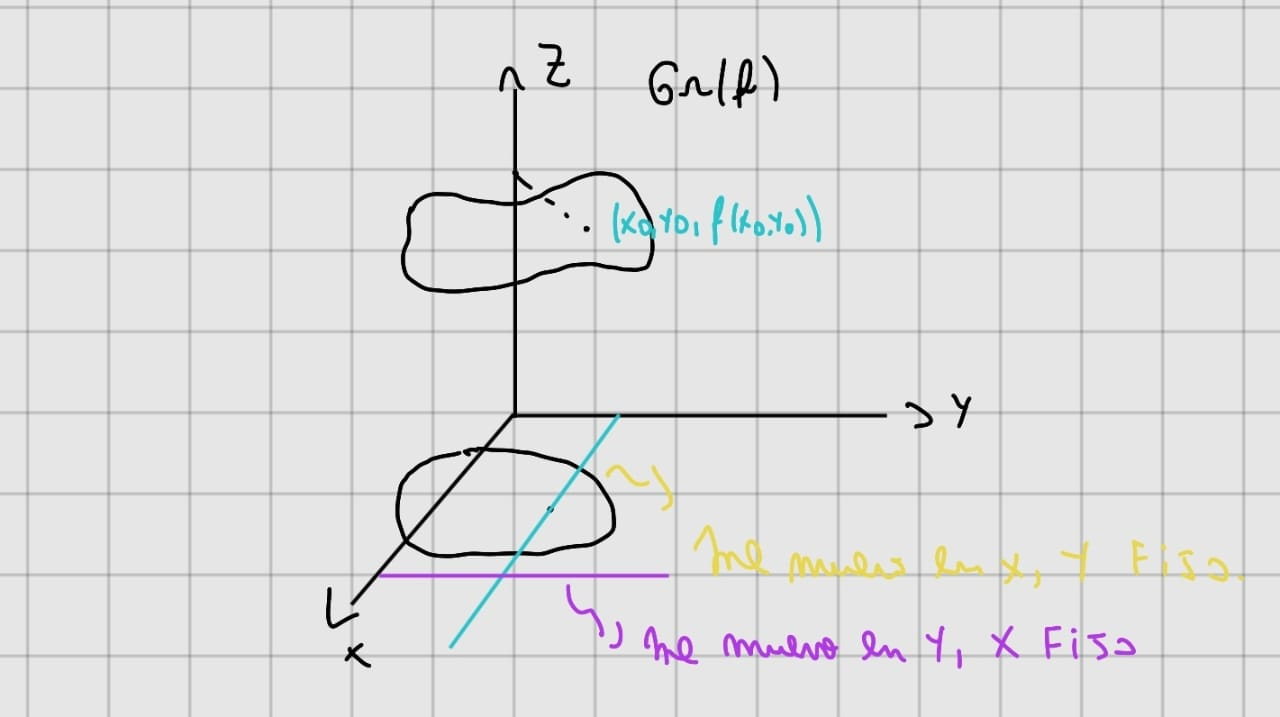
\includegraphics[width=\linewidth]{assets/derivadas_parciales.jpg}
\end{minipage}\]
\textbf{Importante}: El h \textbf{siempre} tiende a 0.
\subsection*{Derivada parcial de f respecto a x}
Sea f $f(x,y)$, la derivada parcial de f respecto a x es:
\[f_{x}(x_{0}, y_{0}) = \lim_{h \to 0} \left(\frac{f(x_{0} + h, y_{0}) - f(x_{0}, y_{0})}{h} \right)\]
\[\frac{\partial f}{\partial x}(x_{0}, y_{0}) = f_{x}(x_{0}, y_{0})\]
Ambas notaciones denotan lo mismo. 
\subsection*{Derivada parcial de f respecto a y}
Sea f $f(x,y)$, la derivada parcial de f respecto de y es: 
\[f_{y}(x_{0}, y_{0}) = \lim_{h \to 0} \left(\frac{f(x_{0}, y_{0} + h) - f(x_{0}, y_{0})}{h} \right)\]
\[\frac{\partial f}{\partial y}(x_{0}, y_{0}) = f_{y}(x_{0}, y_{0})\]
En ambos casos, la derivada parcial existe si el límite existe. \\
Lo único que cambia de ambas es que cuando queremos ver la derivada parcial de f respecto a una variable, a esa variable le sumamos h. Lo demás es igual, cambia la notación porque ahora vamos a evaluar todo en base a esa variable pero nada más que eso. \\
Véase \hyperref[subsec:derivadas_parciales]{\underline{\textbf{anexo}}} para ver ejemplos de ejercicios de derivadas parciales.
\section*{Vector Gradiente}
Es un vector que posee las dos derivadas parciales y se denota de la siguiente manera
\[\triangledown f(x,y) = (f_{x}(x,y), f_{y}(x,y))\]
Considerando el primer ejemplo que resolvimos en la sección anterior que se encuentra en el anexo podemos ver que el vector gradiente para todo x, y es el siguiente: $\triangledown f(x, y) = (\frac{1}{x}, \frac{-1}{1+y})$
\section*{Derivadas Direccionales}
Sea $v \in \float^{2}, \longitud{v} = 1, v \neq 0$ definimos la derivada direccional f en $(x_{0}, y_{0})$ \\ 
$\frac{\partial f}{\partial v}(x_{0}, y_{0}) = D_{v}(x_{0}, y_{0}) = \lim_{t \to 0} \left(\frac{f((x_{0}, y_{0}) + t(a, b)) - f(x_{0}, y_{0})}{t} \right) $ siempre que este límite exista. \\
Esto siempre se hace por definición, pero si tenemos la información de que es \textbf{diferenciable} podemos usar el Teorema de la Diferenciabilidad. 
\subsection*{Aclaración acerca de analizar derivadas direccionales en \textbf{todos} los puntos}
Cuando nos piden analizar todas las derivadas direccionales, y aplicamos la definición y nos quedó algun caso fuera, como por ejemplo, si $b = 0$ se rompe ese caso hay que verlo aparte. \\
Curiosamente, como los vectores son de norma 1, si el caso que nos quedó fuera es $b=0$ el único caso de norma 1 que es sería $\frac{\partial f}{\partial x}$ pues, esta derivada tiene como dirección (1,0). \\
La idea de estos ejercicios es tratar de \textbf{todas las maneras} posibles ver que el límite no se rompa. Normalmente en el denominador queda algún tipo de suma que evita que algo se rompa del todo, pero si solamente tenemos una variable en el denominador, a toda costa hay que evitar que sea 0, y si lo es, hay que analizarlo aparte. 
\subsubsection{Calcular \textbf{todas las derivadas direccionales} y analizar diferenciabilidad}
\[\begin{minipage}[b]{0.7\textwidth}
    \includegraphics[width=\linewidth]{assets/derivadas_direccionales_diferenciabilidad.png}
\end{minipage}\]
\textbf{Inciso a}: \\
Cuando venis haciendo las guías la mayoría salen muy fácil, pero este particularmente asusta porque tenés varias cosas: 
\begin{itemize}
    \item No podés aplicar el mejor caso, tener algo de la forma $\frac{a^{2}}{a^{2} + b^{2}}$
    \item Tenés módulos.
\end{itemize}
Lo primero que hay que recordar es ¿qué son las derivadas direccionales? \\
Recordemos que las derivadas direccionales son vectores de la forma $v = (a,b)$ y que tienen norma 1, es decir $\longitud{\longitud{v}} = 1$. \\
Recordar que cuando hablamos en vectores, hablamos de norma, en números hablamos de módulo. \\
Sabiendo estas cosas ¿qué es lo que podríamos esperar de este límite?, que como nos piden \textbf{probar que existen todas}, si llega un caso donde decimos que se indefine, entonces tenemos que analizarlo aparte. \\
Si comenzamos aplicando el límite de Derivadas Direccionales nos queda algo que nos puede dar un poco de terror, pero acordarse que la idea para sacarnos los módulos de encima es hacer límites laterales \textbf{a una} de las variables, usar alguna que otra curva y ver que no se rompa. \\
El objetivo entonces, es que nunca se indefina. Si se indefine, lo vemos aparte. \\
$\lim_{t \to 0} \left(\frac{f((x_{0}, y_{0}) + t(a, b)) - f(x_{0}, y_{0})}{t} \right) = \lim_{t \to 0} \left(\frac{f(ta, tb) - f(0, 0)}{t} \right)  = \lim_{t \to 0} \left(\frac{\frac{2((ta)^{2} + (tb)^{2}) \longitud{ta} tb}{(ta)^{6} + \longitud{tb}^{3}}}{t} \right) $ \\
A partir de este límite, nos queremos sacar de encima los módulos así que veamos los límites laterales y debemos esperar que claramente den lo mismo. Si dan diferente, no existe ninguna derivada direccional. \\
$\lim_{t \to 0^{+}} \left(\frac{\frac{2((ta)^{2} + (ta)^{2}) ta tb}{(ta)^{6} + (tb)^{3}}}{t} \right) = \lim_{t \to 0^{+}} \left(\frac{2((ta)^{2} + (ta)^{2}) ta tb}{t((ta)^{6} + (tb)^{3})} \right) = \lim_{t \to 0^{+}} \left(\frac{(2t^{2}a^{2} + 2t^{2}b^{2}) \textcolor{red}{t^{2}}ab}{\textcolor{red}{t}((ta)^{6} + (tb)^{3})} \right) = \lim_{t \to 0^{+}} \left(\frac{(2t^{2}a^{2} + 2t^{2}b^{2}) tab}{(ta)^{6} + (tb)^{3}} \right) $ \\
$= \lim_{t \to 0^{+}} \left(\frac{(2t^{2}a^{2} + 2t^{2}b^{2}) \textcolor{red}{t}ab}{\textcolor{red}{t^{3}}(t^{3}a^{6} + b^{3})} \right) = \lim_{t \to 0^{+}} \left(\frac{(2t^{2}a^{2} + 2t^{2}b^{2})ab}{t^{2}(t^{3}a^{6} + b^{3})} \right) = \lim_{t \to 0^{+}} \left(\frac{\textcolor{red}{t^{2}}(2a^{2} + 2b^{2})ab}{\textcolor{red}{t^{2}}(t^{2}a^{6} + b^{3})} \right) = \lim_{t \to 0^{+}} \left(\frac{2(a^{2} + b^{2})ab}{t^{2}a^{6} + b^{3}} \right)$  \\
Ahora paremos la pelota y veamos el límite. Evaluemos el límite con $t \rightarrow 0^{+}$, nos queda $\lim_{t \to 0^{+}} \left(\frac{2(a^{2} + b^{2})ab}{b^{3}} \right)$ \\
¿Qué es lo que tiene que pasar para que el límite se indefina? b debe ser = 0. \\
Ahora, cualquier otro caso vale. Entonces, valen todas las derivadas direccionales por ahora \textbf{excepto} el vector norma 1 cuando $b=0$ que sería curiosamente, la derivada parcial $(1,0)$ osea $\frac{\partial f}{\partial x}$. 
Si hacemos de ambos lados, llegamos prácticamente a lo mismo. Si se llegase a otra condición \textbf{el límite no existe}. \\
Entonces hasta ahora, probamos que valen todas las derivadas direccionales en el (0,0) excepto el vector $(1,0)$ pero como nos lo piden aparte, veamos si esa derivada existe. \\
$\lim_{h \to 0} \left(\frac{f(h + x_{0}, y_{0}) - f(x_{0}, y_{0})}{h} \right) = \lim_{h \to 0} \left(\frac{f(h, 0)}{h} \right) = \lim_{h \to 0} \left(\frac{\frac{2(h^{2} + 0^{2}) \longitud{h} y}{h^{6} + \longitud{0}^{3}}}{h} \right) = \lim_{h \to 0} \left(\frac{0}{h^{7}} \right) = 0  $ \\
Luego, como el límite dió 0 sin ningun tipo de problema, la derivada parcial existe y es 0. \\
Por lo tanto, existen todas las derivadas direccionales en el punto (0,0). \\
\textbf{Inciso b}: Analicemos la diferenciabilidad de f en (0,0). Recordemos que el concepto de diferenciabilidad es lo mismo que calcular derivabilidad en una variable. \\
Entonces, que una función sea diferenciable implica que tenga un plano tangente, sus derivadas parciales y además de eso, también que es continua en ese punto. Una función \textbf{no puede ser diferenciable} en un punto si no es continua en ese punto. \\
Sin embargo, es raro que tengamos que evaluar continuidad porque seria un poco más largo, así que si te dicen que analices la diferenciabilidad, considerá que es continua (preguntalo igual). \\
Calculemos primero la derivada parcial que nos falta, es decir $\frac{\partial f}{\partial y}$ y tenemos suerte de que la de x ya la hayamos calculado. \\
Por suerte, ambas dan 0, entonces, ya podemos armar el hipotético plano tangente. Sí, hipotético, porque no es el plano tangente hasta que probemos que es diferenciable. \\
El plano tangente se arma con $f(0, 0) + f_{x}(x-x_{0}) + f_{y}(y-y_{0})$. En nuestro caso es $z = 0$. \\
Entonces, el límite para probar diferenciabilidad es de la siguiente forma: $\lim_{(x, y) \to (0,0)} \left(\frac{f(x,y) - [f(0, 0) + f_{x}(x-x_{0}) + f_{y}(y-y_{0})]}{\longitud{\longitud{(x,y) - (x_{0}, y_{0})}}} \right)$ y debería dar 0. \\
Luego, $\lim_{(x, y) \to (0,0)} \left(\frac{\frac{2(x^{2} + y^{2})\longitud{x} y}{x^{6} + \longitud{y}^{3}}}{\longitud{\longitud{(x,y)}}} \right) = \lim_{(x, y) \to (0,0)} \left(\frac{2(x^{2} + y^{2})\longitud{x} y}{\longitud{\longitud{(x,y)}} * x^{6} + \longitud{y}^{3}} \right)$ \\
Misma estrategia que antes. Saquémosnos de encima los módulos, veamos los laterales con la recta y = x porque intuyo que no existe porque el grado del denominador es mucho más grande que el del numerador. \\
$\lim_{x \to 0^{+}} \left(\frac{2(x^{2} + x^{2})x x}{\longitud{\longitud{(x,y)}} * x^{6} + \longitud{x}^{3}} \right) = \lim_{x \to 0^{+}} \left(\frac{2(x^{2} + x^{2})x^{2}}{\sqrt{2x^{2}} * (x^{6} + \longitud{x}^{3})} \right) = \lim_{x \to 0^{+}} \left(\frac{4x^{2} * x^{2}}{\sqrt{2} \longitud{x^{2}} * (x^{6} + x^{3})} \right) = \lim_{x \to 0^{+}} \left(\frac{4x^{4}}{\sqrt{2} x * (x^{6} + x^{3})} \right)    $ \\
$\lim_{x \to 0^{+}} \left(\frac{4x^{3}}{\sqrt{2} * (x^{6} + x^{3})} \right) = \lim_{x \to 0^{+}} \left(\frac{4x^{3}}{\sqrt{2} * (x^{3}(x^{3} + 1))} \right) =  \lim_{x \to 0^{+}} \left(\frac{4}{\sqrt{2} * (x^{3} + 1)} \right) $ \\
Si ahora evaluamos el límite nos queda $\lim_{x \to 0^{+}} \left(\frac{4}{\sqrt{2}} \right)$ y esto claramente no es 0. Por lo tanto, no es diferenciable en (0,0) \\
\textbf{Conclusión}: Es realmente útil utilizar límites laterales por un lado, y además probar por curvas/rectas. 
\subsection*{Derivadas Direccionales con Ángulos}
En este tipo de casos hay que pensar que cuando dibujamos un ángulo, indirectamente podría haber un vector que salga con esa inclinación. \\
Por lo tanto, podemos recordar las definiciones de
\[
\begin{cases}
x = r * cos(\Theta) \\
y = r * sen(\Theta)
\end{cases}
\]
Pero acá el rol de x lo toma \textbf{a} y el rol de y lo toma \textbf{b} donde $v=(a,b)$. \\
¿Qué es r? Recordemos que r era el radio/largo. En este caso va a ser \textbf{siempre 1} si hablamos del vector normalizado. \\
Lo demás es exactamente igual, una vez que encontramos el vector queda hacer las derivadas parciales, generar el gradiente, evaluar en el punto dado y hacer el producto escalar entre el gradiente evaluado en el punto y el vector. 
\subsection*{Relación entre las Derivadas Direccionales y Derivadas Parciales}
Las Derivadas Parciales son literalmente Derivadas Direccionales pues cuando estamos derivando en base a x estamos usando el vector director de norma 1 (1,0) y cuando lo hacemos en base a y estamos usando el vector director de norma 1 (0, 1): 
\begin{itemize}
    \item $\frac{\partial f}{\partial x}(x_{0}, y_{0}) = D_{(1, 0)} f (x_{0}, y_{0})$
    \begin{itemize}
        \item $\frac{\partial f}{\partial(1,0)} (x_{0}, y_{0})$
    \end{itemize}
    \item $\frac{\partial f}{\partial y}(x_{0}, y_{0}) = D_{(0, 1)} f (x_{0}, y_{0})$
    \begin{itemize}
        \item $\frac{\partial f}{\partial(0, 1)} (x_{0}, y_{0})$
    \end{itemize}
\end{itemize}
Véase \hyperref[subsec:derivadas_direccionales_ej]{\textbf{\underline{anexo}}} para ver ejemplos.
\section*{Derivadas de Orden Superior}
Ejemplo: Sea $f(x,y) = x^{3}y^{2} + 2x - y^{4}$ calculemos sus derivadas parciales. 
\begin{itemize}
    \item $\frac{\partial f}{\partial x}(x,y) = 3x^{2}y^{2} + 2$
    \item $\frac{\partial f}{\partial y}(x,y) = 3x^{2}2y - 4y^{3}$
\end{itemize}
Entonces ahora ¿cuántas derivadas parciales podemos calcular de ambas funciones nuevas?, esto lo conocemos como derivadas de orden superior.
\begin{itemize}
    \item $(f_{x})_{x}(x, y) = \frac{\partial}{\partial x}(\frac{\partial f}{\partial x})(x,y) = 6xy^{2}$
    \item $(f_{x})_{y}(x, y) = \frac{\partial}{\partial y}(\frac{\partial f}{\partial x})(x,y) = 6x^{2}y$
    \item $(f_{y})_{x}(x, y) = \frac{\partial}{\partial x}(\frac{\partial f}{\partial y})(x,y) = 6x^{2}y$
    \item $(f_{y})_{y}(x, y) = \frac{\partial}{\partial y}(\frac{\partial f}{\partial y})(x,y) = 2x^{3}-12y^{2}$
\end{itemize}
\section*{Funciones de clase $C^{k}$}
Son un conjunto especial de funciones que se caracterizan por ser \textbf{continuas y tener derivadas continuas hasta el k-ésimo orden}.
\subsection*{Teorema}
Si $f:D \subseteq \float^{2} \implies \float$ es de clase $C'(D) \implies f$ es diferenciable en $D$.
\[\begin{minipage}[b]{0.6\textwidth}
    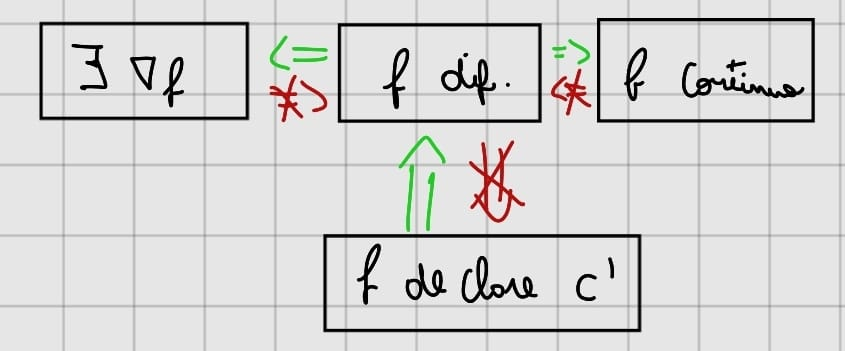
\includegraphics[width=\linewidth]{assets/relacion_diferenciabilidad_continua_clases.jpg}
\end{minipage}\]
\section*{Teorema de Clairaut}
Si $f:D \subseteq \float^{2} \rightarrow \float$ y existen $f_{xy}, \ f_{yx}$ y son continuas en D. Entonces $f_{xy}=(x_{0}, y_{0}) = f_{yx}(x_{0}, y_{0})$ $\forall(x_{0}, y_{0}) \in D$ \\
En el ejemplo que vimos en Derivadas de Orden Superior esto sucede porque $(f_{x})_{y} = (f_{y})_{x}$, es decir, las derivadas cruzadas dan igual.
\section*{Función Lineal en $\float^{3}$}
$L(x,y) = a(x-x_{0}) + b(y-y_{0})+f(x_{0}, y_{0})$ \\
$L:\float^{2} \rightarrow \float \ f:D\subseteq \float^{2} (x_{0}, y_{0}) \in D$ \\
\textbf{Importante}: a y b son las dos pendientes de la función lineal.
\section*{Diferenciabilidad}
Sea $f:D \subseteq \float^{2} \rightarrow \float \ (x_{0}, y_{0}) \in D$ es diferenciable en $(x_{0}, y_{0})$ si $\exists a,\ b \in \float$ tal que 
\[\lim_{(x,y) \to (x_{0}, y_{0})} \left(\frac{f(x, y) - f(x_{0}, y_{0}) - a(x - x_{0}) - b(x - y_{0})}{\longitud{\longitud{(x, y) - (x_{0}, y_{0})}}} \right) = 0\]
\textbf{Consideraciones importantes}
\begin{itemize}
    \item Como el límite es 0, esto quiere decir que el numerador tiende más rápido al cero.
    \item f(x,y) se acerca al plano tangente.
    \item $\longitud{\longitud{(x,y) - (x_{0}, y_{0})}}$ tiende a cero. 
\end{itemize}
\textbf{Nota}: En una variable lo conocemos como derivada, y existe una recta tangente. Acá se lo conoce como Diferenciabilidad y existe un plano tangente. \\
\textbf{Nota}: Como en todo límite, acá podemos usar todo lo que conocemos de límites laterales, l'hopital (cuando sea posible) para chequear y efectivamente romper la diferenciabilidad. \\
\subsection*{Teorema de la Diferenciabilidad}
Sea $f:D \subseteq \float^{2} \rightarrow \float$ diferenciable en $(x_{0}, y_{0}) \in D$ entonces vale que 
\begin{itemize}
    \item $a = f_{x}(x_{0}, y_{0}), b = f_{y}(x_{0}, y_{0})$
    \item $ \frac{\partial f}{\partial v}(x_{0},y_{0}) = \triangledown f (x_{0}, y_{0}) * \frac{v}{\longitud{\longitud{v}}} = \frac{\partial f}{\partial x}(x_{0}, y_{0}) * a + \frac{\partial f}{\partial y}(x_{0}, y_{0})*b$
\end{itemize} 
\textbf{Nota}: $(x_{0}, y_{0}) + t(a,b)$ donde v=(a, b) 
\subsection*{Teorema de Diferenciabilidad $\&$ Continuidad}
Sea $f:D\subseteq \float^{2} \rightarrow \float$ y $P_{0} = (x_{0}, y_{0}) \in D$ si sucede que f es diferenciable en $p_{0}$ entonces, f es continua en $p_{0}$.
\subsection*{Álgebra de Diferenciabilidad}
Valen exactamente las mismas que las de las derivadas. \\
Sea $f, g: D \subseteq \float^{2} \implies \float$, $p_{0} \in D \ \backslash \ \exists \ \triangledown f(p_{0}), \triangledown g(p_{0})$ 
\begin{itemize}
    \item Linealidad: $\alpha, \beta \in \float \implies \exists \ \triangledown (\alpha f + \beta g) (p_{0})$ y $\triangledown(\alpha f + \beta g) = \alpha \triangledown f + \beta \triangledown g$
    \item Producto: $\triangledown (f, g)(p_{0}) = \triangledown f(p_{0}) * g(p_{0}) + f(p_{0}) * \triangledown g (p_{0})$
    \item Cociente: $g(p_{0}) \neq 0 \implies \triangledown(f/g)(p_{0}) = \frac{\triangledown f(p_{0}) * g(p_{0}) - f(p_{0}) * \triangledown g(p_{0})}{g(p_{0})^{2}}$
\end{itemize}
Véase \hyperref[subsec:diferenciabilidad_continuidad_mas]{\textbf{\underline{anexo}}} para ver ejercicios donde vemos continuidad, dominio, diferenciabilidad y más.
\subsection*{Relación entre Gradiente, Diferenciabilidad, Continuidad y Clases}
\[\begin{minipage}[b]{0.8\textwidth}
    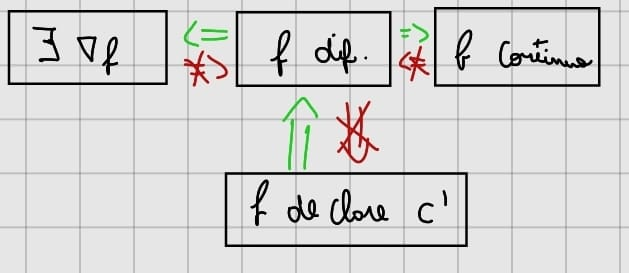
\includegraphics[width=\linewidth]{assets/relacion_continuidad_diferenciabilidad.jpg}
\end{minipage}\]
\begin{itemize}
    \item Si existe el gradiente (o la derivada), la función es diferenciable.
    \item Si la función es diferenciable, entonces es continua.
    \item Una función continua no necesariamente es diferenciable.
    \item Una función diferenciable no necesariamente es de clase C1 (su derivada puede no ser continua).
    \item Si una función es de clase C1 entonces es diferenciable y su derivada es continua.
    \item Si una función no es continua en un punto, entonces no es diferenciable en ese punto, es decir, no existen las derivadas parciales ni plano tangente, ni la diferenciabilidad.
\end{itemize}
\section*{Plano Tangente}
Sea $f:D \subseteq \float^{2} \rightarrow \float$ \textbf{diferenciable} en $P_{0} \in D$ 
\[f(x_{0}, y_{0}) + f_{x}(x_{0}, y_{0})(x-x_{0})+f_{y}(x_{0}, y_{0})(y-y_{0}) = f(x_{0}, y_{0}) + \triangledown f(x_{0}, y_{0})(x-x_{0})(y-y_{0})\] 
El plano tangente existe solo si es Diferenciable. Esto quiere decir que si bien podemos plantear la ecuación de un hipotético plano, la forma de validar que efectivamente exista es que el límite de Diferenciabilidad de 0. \\
Si es Diferenciable, y encontramos un plano, entonces ese plano es único. 
\section*{Regla de la Cadena}
\subsection*{Regla de la Cadena en 1 Variable}
Cuando teníamos una sola variable, la regla de la cadena en derivadas tenía esta pinta $f'(x(t_{0})) * x'(t_{0})$ y en forma de derivadas parciales se ve de esta manera $y=f(x)$ y $x=x(t)$ 
\[\frac{dy}{dt} = \frac{dy}{dx} * \frac{dx}{dt} \]
donde $dx = f'(x)$ y $dt = x'(t)$ 
\subsection*{Regla de la Cadena en 2 Variables}
Tiene esta pinta $z = f(x,y)$ $x=x(t)$ $y=y(t)$ \\
¿Cómo calculamos $\frac{dz}{dt}$?
\[\frac{d}{dt}[f(x(t), y(t))] = f_{x}(x, y) * x' + f_{y}(x,y) * y' = \triangledown f(x,y) * (x', y')\]
\textbf{Importante}: Si $r(t) = (x(t), y(t))$ entonces $\triangledown f(x,y) * (x', y') = \triangledown f (r) * r'$ donde $r'(t)$ es $(x', y')$ y r es $(x,y)$
\subsection*{Diagrama del Árbol}
Cuando queremos calcular la derivada de una función que depende de 2 variables o más y que a su vez esas variables dependan de más de una, solemos usar el diagrama del árbol. \\
Ej.: Si tengo $z=f(x,y)$ con $x=x(u, v), y=y(u,v)$ ¿cómo calculamos $Z_{u}$ y $Z_{v}$? \\
\begin{itemize}
\item La raíz del árbol va a ser lo que queremos calcular, en este caso z.
\item Las ramas de la raíz serán las variables que necesito enviar para calcular z. En este caso, x e y.
\item Luego, las ramas de x e y son justamente las variables de las que dependen. En este caso, x depende de u y v y lo mismo sucede con y.
\end{itemize}
\[\begin{minipage}[b]{0.9\textwidth}
    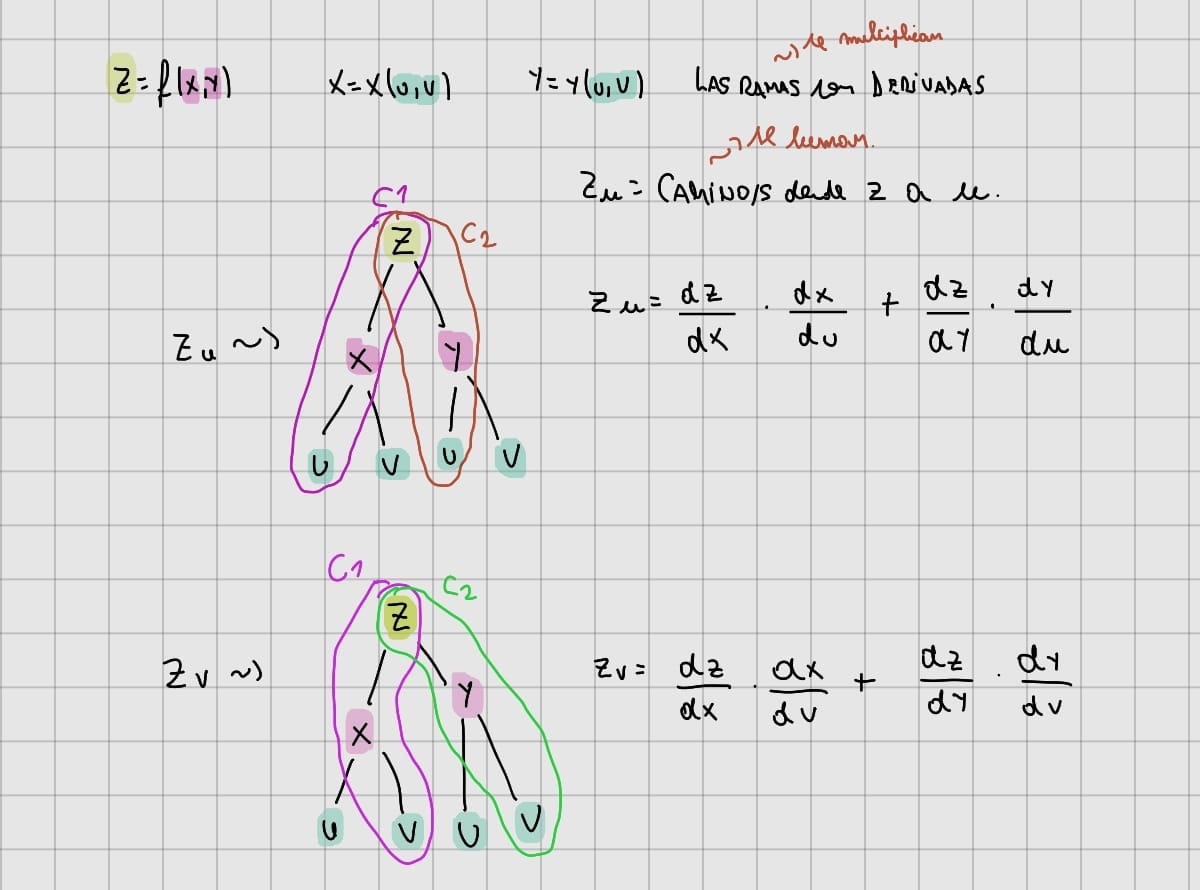
\includegraphics[width=\linewidth]{assets/arbol_derivadas.jpg}
\end{minipage}\]
Otro ejemplo 
\[\begin{minipage}[b]{0.6\textwidth}
    \includegraphics[width=\linewidth]{assets/regla_cadena_arbol.png}
\end{minipage}\]
\section*{Anexo}
\subsection*{Esferas}
\label{subsec:completar_cuadrados_esfera}
Complete y lleve a una fórmula conocida: $x^{2} + y^{2} + z^{2} + 8x - 6y + 16$ 
\begin{itemize}
    \item Reordeno: $x^{2} + 8x + y^{2} - 6y +z^{2} = -16$ 
    \item Completo cuadrados, los valores que tienen la variable (sin exponente), hago $(num/2)^{2}$.
    \begin{itemize}
        \item $(x^{2} + 8x + 16) + (y^{2} - 6y + 9) + z^{2} - 16 - 9 = -16$
        \item Nótese que como nos inventamos términos para completar cuadrados, tenemos que restarlos.
    \end{itemize}
    \item Reordeno: $(x^{2} + 8x + 16) + (y^{2} - 6y + 9) + z^{2} = -16 + 16 + 9$
    \item Para agrupar un cuadrado, el numero que no tiene variable, tengo que aplicarle la raíz cuadrada. Luego, el símbolo que los separa es el signo del coeficiente que tiene variable grado uno.
    \begin{itemize}
        \item $(x+4)^{2} + (y-3)^{2} + z^{2} = 9$
    \end{itemize}
    \item Por último, como el radio está elevado al cuadrado lo reducimos $(x+4)^{2} + (y-3)^{2} + z^{2} = 3$
    \item El resultado entonces, es una Esfera en $\float^{3}$ con centro = (-4, 3, 0) y radio = 3
    \item Si se quisiera verificar si está bien, podemos desarrollar todos los cuadrados y deberíamos volver a la expresión original.
\end{itemize}
\subsection*{Completar Cuadrados}
Adjunto otro ejercicio que es de cónicas, pero acá tuve que completar cuadrados de una manera ligeramente diferente. \\
La forma de encararlo fue dejar el valor que esta solo del lado positivo. \\
Luego, como tuve que sacar factor común de las letras, al tener que completar los cuadrados lo que le tengo que restar es el factor común * el valor que agregué. Eso es lo que termino restando. 
\[\begin{minipage}[b]{0.9\textwidth}
    \includegraphics[width=\linewidth]{assets/completar_cuadrados.png}
\end{minipage}\]
\subsection*{Planos}
\label{subsec:ejercicios_planos}
\textbf{1}. Hallar la ecuación implícita del plano $\pi$ cuya normal sea $N=(-3, 0, 4)$ y que pasa por el punto $P=(2, 1, 1)$ \\
Recordemos como podemos armar un plano. Para poder armar un plano necesitamos un vector normal y un punto de paso. \\
Por lo tanto, este ejercicio es bastante simple, podemos simplemente aplicar la fórmula de $\pi:ax+by+cz = d$ \\
Entonces, nos quedaría algo así: $ \pi:-3x + 0y + 4z = d$ \\
Ahora ¿como calculo d?, podemos calcular d evalúando el punto $P$ en el plano. \\
Por lo tanto $d=-3(2) + 4(1) \equiv d = -2$ \\
Entonces, el plano $\pi:-3x+4z=-2$ \\

\textbf{2}. Dados los puntos $A=(1, 2, 3), B=(1,0,1) \ y \ C=(4, -1, 2)$ encuentre el plano. \\
Recordemos como podemos armar un plano. Para poder armar un plano necesitamos un vector normal y un punto de paso. \\
¿Tenemos la normal? No. ¿Como podemos calcularla? La manera de calcular un vector normal sería hacer el producto cruz entre dos vectores directores. \\
Por lo tanto, calculemos nuestros dos vectores directores $ \bar{AB} = (0, -2, -2)$ luego $\bar{BC} = (3, -1, 1)$ \\
\textbf{Nota}: Sería lo mismo calcular AB y BC que AB Y AC.
Ahora lo que podemos hacer es una vez que tenemos las dos direcciones podemos buscar con el producto cruz, un vector perpendicular que hará de nuestra normal. \\
PD: Recordemos que $A x B = - (B x A)$. Por lo tanto da igual que orden pongamos los vectores.
\[
\begin{pmatrix}
\hat{i} & \hat{j} & \hat{k} \\
0 & -2 & -2\\
3 & -1 & 1
\end{pmatrix}
\]
Nuestro vector normal N termina siendo N = $(-4, 6, 6)$ \\
¿Ahora qué nos falta? Un punto. Entonces podemos elegir cualquiera de los puntos A, B, C (xq las rectas estarían contenidas en el plano) \\
Si quisieramos verificar si efectivamente la normal nos dió bien, podemos calcular el producto escalar de $N * AB$ y $N * BC$ y ambos deberían dar 0. \\
Entonces, ahora por último hacemos lo mismo que en ejercicio anterior. $\pi:-4x+6y+6z=d \implies d=-4(1)+6(0)+6(1) \implies d = 2$ \\
Finalizamos, juntando la ecuación $\pi:-4x+6y+6z=2 \equiv \pi:-2x+3y+3z=1$ 
\subsection*{Rectas $\&$ Rectas y Planos}
\label{subsec:ejercicios_rectas_planos}
\textbf{1}. Dadas la recta $L:t(1, 1, 1) + (3, 0, 4)$ y el plano $\pi:2x-y+5z=10$ halle $L \cap \pi$. \\
Recordemos qué significa que una recta pueda intersecarse con un plano: que una recta pueda intersecarse con un plano o al revés significa que existe al menos un punto que tienen en común. \\
Con esto quiero decir que el punto que encontremos debe verificar tanto el plano como la recta. \\
Como tenemos que encontrar UN PUNTO necesitamos encontrar la fórmula generadora de puntos de la recta o el plano. \\
En este caso, como tenemos la recta en parámetrica y el plano en implícita nos conviene más fácil pasar la parámetrica y ver qué pinta tienen los puntos. \\
Entonces, si pasamos L a parámetrica nos queda: $(t+3, t, t+4)$ entonces $x=(t+3), y=t, z=t+4$ \\
Ahora, coloquemos lo que acabamos de encontrar en el plano, esto nos dará la variable $t$ para la recta. Como este t nos lo da después de meterlo el punto de la recta en el plano, cuando reemplacemos en el punto genérico con el t que encontramos, entonces ese punto será el de la intersección del plano y la recta.  \\
$\pi:2(t+3)-(t)+5(t+4)=10 \equiv \pi:2t+6-t+5t+20=20 \equiv \pi:t=\frac{-8}{3}$ \\
Ahora, este t lo colocamos en la fórmula genérica de los puntos de la recta: $((\frac{-8}{3}+3), \frac{-8}{3}, \frac{-8}{3}+4)$. \\
Entonces, la intersección es el punto $P=(\frac{1}{3}, \frac{-8}{3}, \frac{4}{3})$ \\
Por lo tanto, verifiquemos ahora, si este punto verifica el plano. \\
$\pi:2(\frac{1}{3}) - (\frac{-8}{3}) + 5(\frac{4}{3}) = 10 \equiv 10 = 10$

Luego, como el punto lo arrojó la recta, y verifica el plano, entonces la intersección $ L \cap \pi = (\frac{1}{3}, \frac{-8}{3}, \frac{4}{3})$ \\

\textbf{2}. Dar la ecuación implícita del plano $\pi$ que contiene a la recta. \\
$L:\alpha(2, 1, 3) + (2, 1, 0)$ y al punto $P=(0, 1, -1)$
Recordemos que si un plano contiene a una recta, todos los puntos de la recta están en el plano. \\
(preguntar qué pasaba si el punto estaba en la recta, qué cambiaba el ejercicio, en este caso no está)
Lo primero que tenemos que ver es si el punto $P \in L$. Si el punto está en la recta, entonces hay infinitos planos. Si el punto NO está en la recta, entonces hay un único plano. \\
Como necesito sí o sí dos vectores directores para mi plano, puedo hacer un vector director de la resta de $QP=(0, 1, -1) - (2, 1, 0) = (-2, 0, -1)$ \\
Entonces ahora hago el producto cruz entre $(2, 1, 3)$ y $(-2, 0, 1)$
\[
\begin{pmatrix}
\hat{i} & \hat{j} & \hat{k} \\
-2 & 0 & -1\\
2 & 1 & 3
\end{pmatrix}
\]
Nuestro vector normal N termina siendo N = $(1, 4, -2)$  \\
Entonces ahora, finalizamos el ejercicio evaluando en la normal el punto P $\pi:x+4y-2z=d$ \\
$d = (0) + 4(1) - 2(-1) \equiv d = 6$ \\
Entonces finalizamos con $\pi:x+4y-2z=6$ \\

\textbf{3}. Dadas las rectas $L_{1}:\alpha(-1, 0, 1) + (4, 3, 2)$ y $L_{2}:\gamma(2, 0, -2) + (0, 0, 1)$. Halle la ecuación implícita del plano $\pi$ que las contiene. \\
Lo primero que vemos es que tenemos dos rectas. Necesitamos de alguna manera un vector normal para el plano. \\
Primero vemos qué relación hay entre las rectas, podemos ver que son paralelas porque si hacemos $(-1, 0, 1) * -2$ nos da $(2, 0, -2)$. \\
Como son paralelas, necesitamos de alguna manera, llegar desde una recta a la otra, para luego, cuando tenemos un punto que llega y combina las rectas, ahí si podemos calcular con el producto cruz el vector normal. \\
\begin{center}
    \begin{minipage}[b]{0.6\textwidth}
        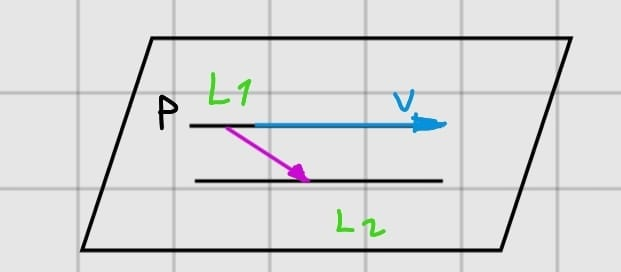
\includegraphics[width=\linewidth]{assets/rectas_paralelas_plano.jpg}
        \centering
        \label{fig:rectas_paralelas_plano}
    \end{minipage}
\end{center}
Entonces, restemos los dos puntos $\bar{PQ}=Q-P=(0, 0,1)-(4,3,2) = (-4, -3, 1)$. \\
Por lo tanto, ahora sí que tenemos dos vectores directores (no paralelos) podemos hacer el producto cruz para calcular la normal del plano.
\[
\begin{pmatrix}
\hat{i} & \hat{j} & \hat{k} \\
-1 & 0 & 1\\
-4 & -3 & -1
\end{pmatrix}
\]
Nuestro vector normal N termina siendo N = $(3, -5, 3)$ \\
Por lo tanto ahora que tenemos el plano $\pi:3x-5y+3z=d$, buscamos el valor de D evaluando cualquier punto de las rectas $d=3(0)-5(0)+3(1)=3$ \\
Luego, el plano resultante $\pi:3x-5y+3z=3$
\subsection*{Pasaje de Coordenadas Cartesianas a Polares y viceversa}
\label{subsec:pasaje_coord_polares_cartesianas}
\[\begin{minipage}[b]{0.9\textwidth}
    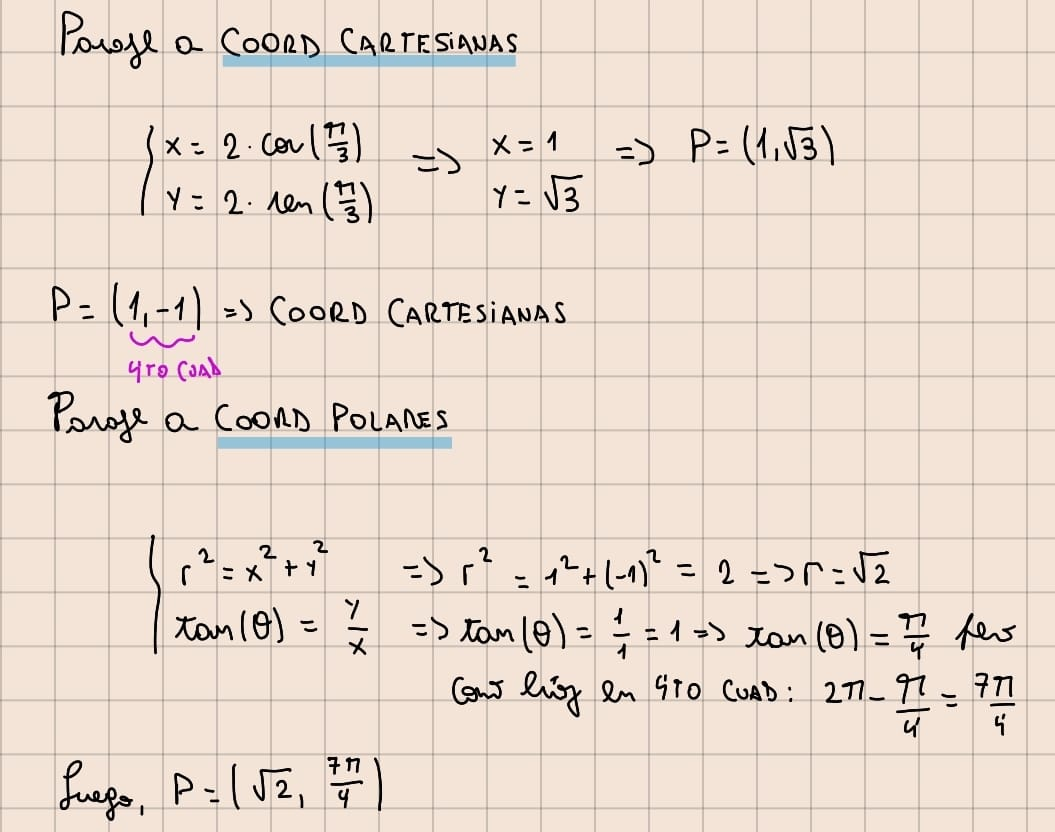
\includegraphics[width=\linewidth]{assets/pasaje_coord_polares_cartesianas.jpg}
\end{minipage}\]
\subsection*{Parametrización}
\label{subsec:curvas_ejemplo}
1. $L: \ (x,y) \ = \ \lambda(2,1) \ + \ (0,1)$ \\
\[
f(t) =
\begin{cases} 
x = 2 \lambda \\
y = \lambda \ + \ 1
\end{cases}
\]
2. ¿Es C gráfico de una función $y = f(x)$?  \\
\[
f(t) =
\begin{cases} 
x = t^{3} - 4t \\
y = t + 1 
\end{cases}
\]
Recordemos que para que una función sea $y = f(x)$ tiene que suceder que para todos los $y$ debe existir un único $x$. \\
Vemos unos casos 
\begin{lstlisting}
    t = 2, x = 0, y = 3
    t = 1, x = -3, y = 2
    t = 0, x = 0, y = 1
    t = -1, x = 3, y = 0
    t = -2, x = 0, y = -1
\end{lstlisting}
No. No es $ y = f(x) $ pues para $x = 0$ existen diferentes valores de y. Si desarrollamos y despejamos nos queda $x = y^{3} - 3y^{2} - y +3$ con $ y \in \float $ \\
3. Grafique la curva C
\[
f(t) =
\begin{cases} 
x = t + 1 \\
y = t^{2}
\end{cases}
\]
Si primero empezamos a darle valores a t vemos que es el gráfico de una parábola y la dirección es de izquierda a derecha
\begin{lstlisting}
    t = -2 x = -1 y = 4
    t = -1, x = 0, y = 1
    t = 0, x = 1, y = 0,
    t = 1, x = 2, y = 1
    t = 2, x = 3, y = 4 
\end{lstlisting}
$y = (x-1)^{2} $. Es una parábola corrida una unidad hacia la derecha.
\[\begin{minipage}[b]{0.4\textwidth}
    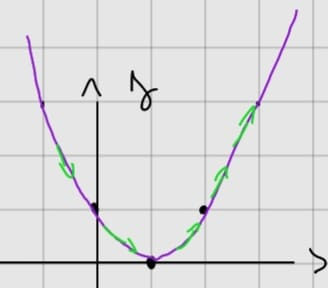
\includegraphics[width=\linewidth]{assets/parabola.jpg}
\end{minipage}\]
4. Hallar una ecuación cartesiana y bosqueje la curva indicando la dirección en que se traza la curva cuando crece el parámetro t. \\
4. 1: $x = \sqrt[]{t} \ y = 1 - t$ \\
4. 2: $x = e^{t} -1 \ y = e^{2t}$ \\
Comenzamos resolviendo $4.1$. Lo que podemos ver es que t > 0 pues de lo contrario x se indefine. \\
Si le damos ciertos valores a t nos queda que la curva va hacia la derecha.
\begin{lstlisting}
    t = 0, x = 0, y = 1
    t = 1, x = 1, y = 0
\end{lstlisting}
Ahora hagamos $4.2$. Lo que podemos ver es que $y = e^{2t}$ es lo mismo que $y = (e^{t})^{2}$. \\
Por lo tanto, como $x + 1 = e^{t}$ entonces $ y = (x+1)^{2}$ \\
En este caso es súper importante entender la función $e$. La función e posee una asíntota en el eje x. En este caso la asíntota está en $y = -1$ pues la función $e^{t} - 1$ tiene la asíntota y corrida una unidad. Si fuese $e^{t} + 4$ la asíntota estaría en y = 4  \\
Por lo tanto, el valor mínimo que puede tener x es -1.
\subsection*{Coordenadas Polares}
Dada la curva $x^{2} + y^{2} = 16$ halle una parametrización. Como es una circunferencia, entonces sabemos que el radio es $4$. Además, las circunferencias se arman con cos / sen. 
\[
f(t) =
\begin{cases} 
x = 4 \ cos(\theta) \\
y = 4 \ sen(\theta) \ con \ 0\le \theta < 2\pi
\end{cases}
\]
Entonces $\alpha(\theta) = \{4 \ cos(\theta), 4 \ sen(\theta)\}$
\subsection*{Elipses}
\label{subsec:elipses_ejercicios}
\[\begin{minipage}[b]{0.7\textwidth}
    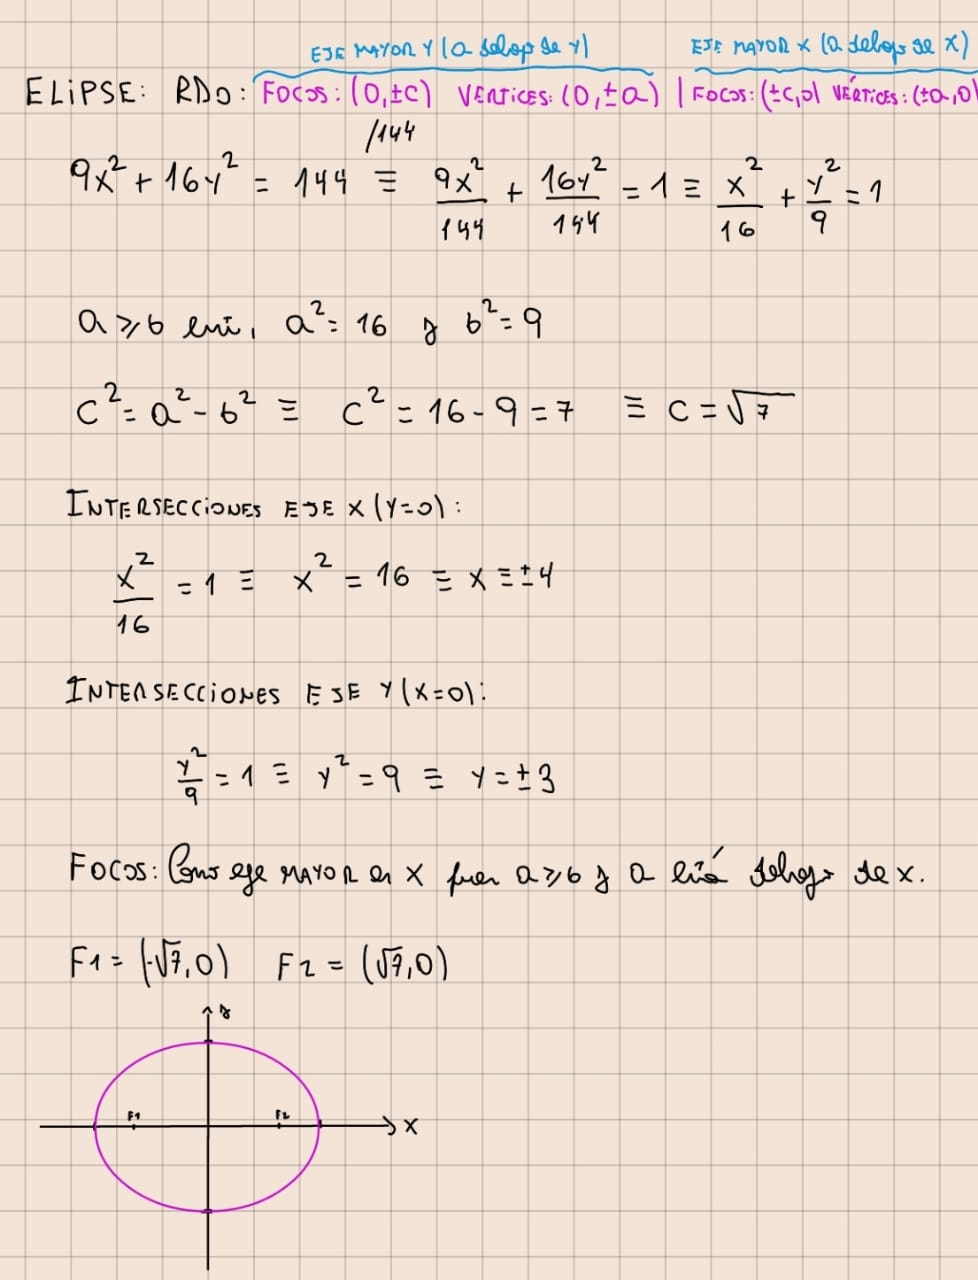
\includegraphics[width=\linewidth]{assets/elipse_1.jpg}
\end{minipage}\]
\[\begin{minipage}[b]{0.7\textwidth}
    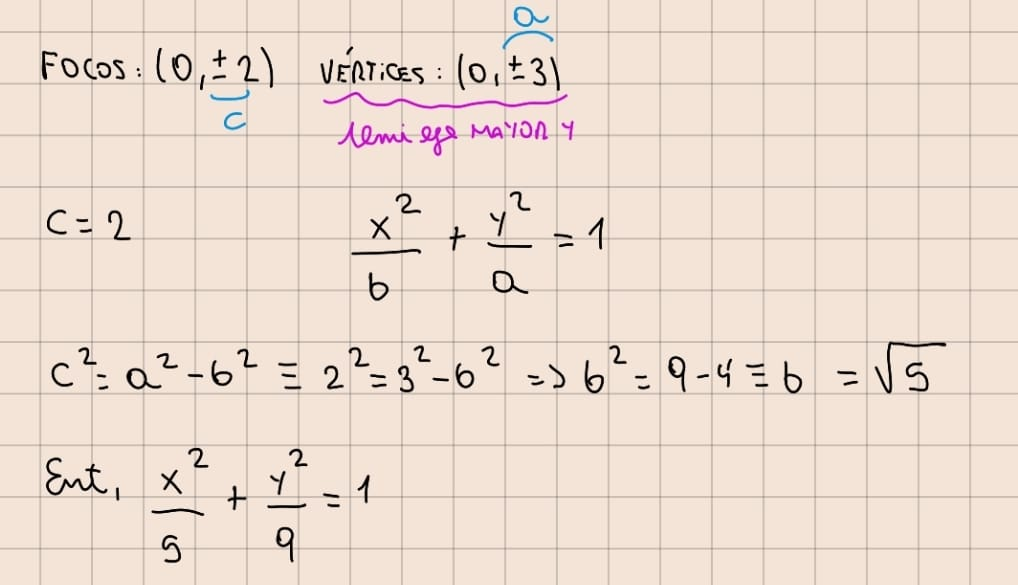
\includegraphics[width=\linewidth]{assets/elipse_2.jpg}
\end{minipage}\]
\textbf{Nota}: Si tengo que pasar una elipse, hipérbola o cualquier otra cosa a una parametrización lo que normalmente se hace es hacer un reemplazo sintáctico. Plantear la parametrización y al final poner el valor real de la variable.
\[\begin{minipage}[b]{0.9\textwidth}
    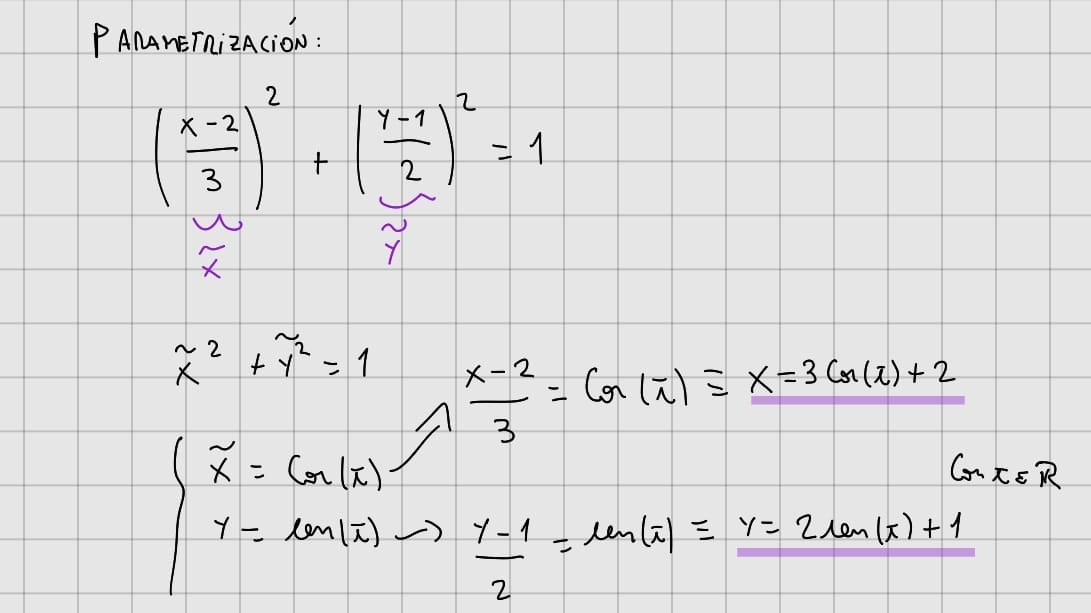
\includegraphics[width=\linewidth]{assets/parametrizacion_elipse.jpg}
\end{minipage}\]
\subsection*{Hipérbolas}
\label{subsec:hiperbolas_ejercicios}
\[\begin{minipage}[b]{0.7\textwidth}
    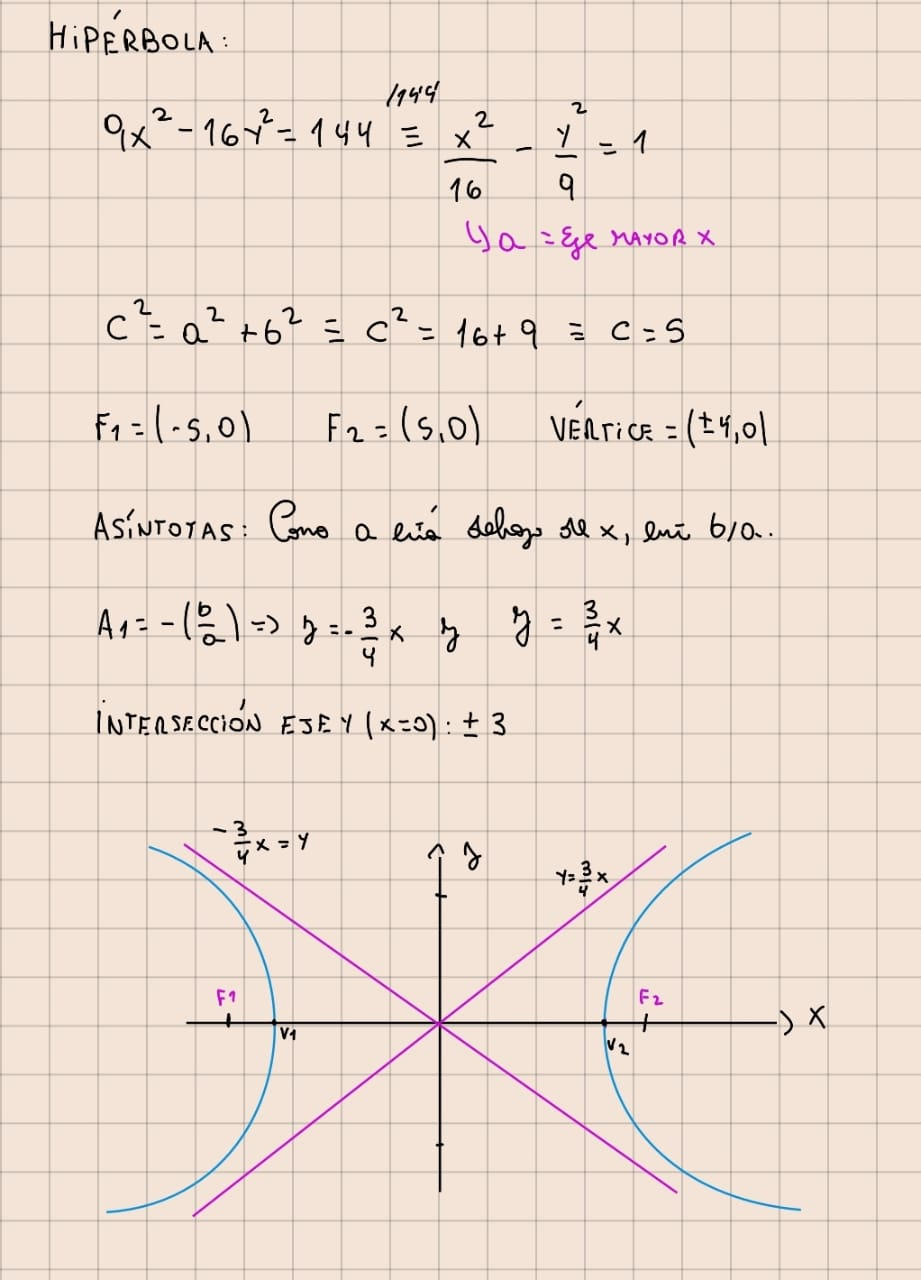
\includegraphics[width=\linewidth]{assets/hiperbola_1.jpg}
\end{minipage}\]
Con cónicas desplazadas y completar cuadrados
\[\begin{minipage}[b]{0.7\textwidth}
    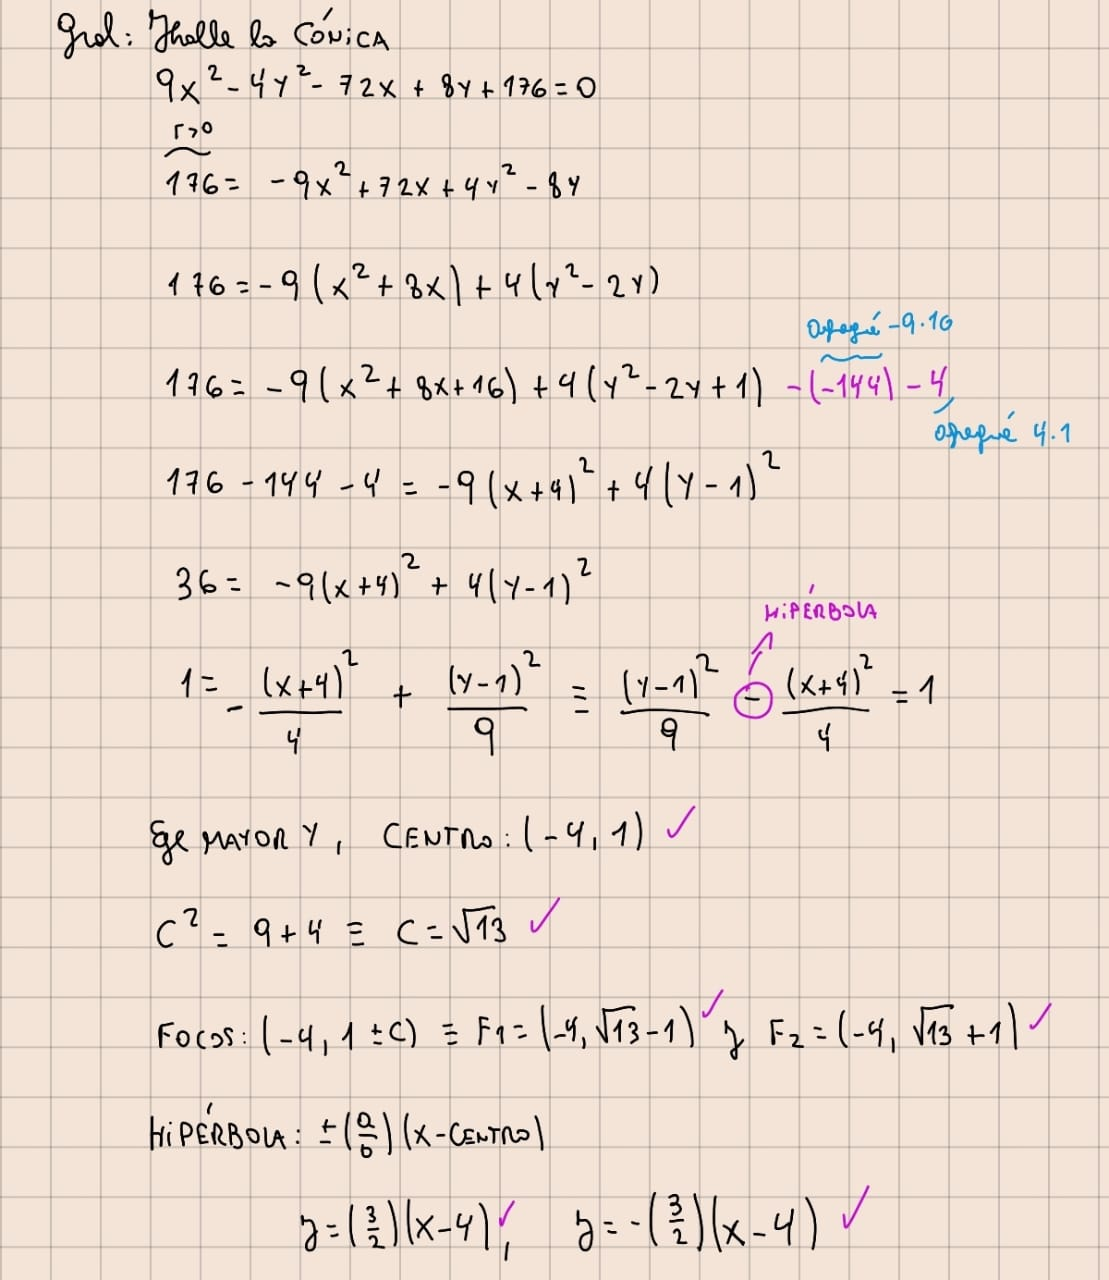
\includegraphics[width=\linewidth]{assets/hiperbola_2.jpg}
\end{minipage}\]
\subsection*{Aplicando Trazas en Superficies}
\label{subsec:trazas_superficies}
Para resolver este ejercicio podemos tomar $z=0$ para empezar y vemos que nos queda la ecuación de una elipse. La dibujamos en el plano de $\float^{3}$. Luego, tomamos $z=k$ y notamos que la constante a lo sumo debe ser 1 porque sino la definición sería erronea, como todos son positivos si $z=2$ falla. Entonces, los k pueden ir desde $-1 \le k \le 1$. Notamos que cortando con un $z=k$ en rango nos da una elipse que cada vez es mas chiquita. \\
Luego, probamos con $y=0$ y esto nos da una circunferencia. \\
Por último, probamos $x=0$ y nos da una elipse. \\
Luego de hacer todas las trazas aproximadas, nos quedaría la figura. \\
Este ejemplo es llamado \textbf{elipsoide}.
\[\begin{minipage}[b]{0.8\textwidth}
    \includegraphics[width=\linewidth]{assets/elipsoide.png}
\end{minipage}\]
\subsection*{Dominio de Funciones}
\label{subsec:dominio_funciones}
1. Calcule el dominio de $ f(x,y) = \sqrt[]{1-2x^{2}-3y^{2}}$ \\
Lo primero que vamos a hacer es reescribir la expresión de la siguiente manera: $ z = \sqrt[]{1-2x^{2}-3y^{2}} $ \\
¿Qué restricciones vemos? ¿Qué valores tomará z? Lo primero que podemos notar es que $z$ siempre será mayor o igual que 0 pues está totalmente atado al cálculo de la raíz. \\
Como necesitamos que el cálculo de la raíz sea mayor o igual a cero para valer, planteemos la desigualdad $\sqrt[]{1-2x^{2}-3y^{2}} \ge 0 \iff 1-2x^{2}-3y^{2} \ge 0 \iff 1 \ge 2x^{2}+3y^{2}  $ ahora como tenemos dos variables, no podemos hacer mucho más. \\
Por lo tanto, $Dom(f) = \{(x, y) \in \float^{2} : 2x^{2} + 3y^{2} \le 1\}$ \\
Entonces, si tuviesemos que graficar, tendríamos que colorear los $2x^{2} + 3y^{2} \le 1$ que estén en $z=0$ o $z=1$ \\
¿Qué curva es? Es una elipse, reescribamos la expresión $ \frac{x^{2}}{\frac{1}{2}} + \frac{y^{2}}{\frac{1}{3}} \le 1 \iff \frac{x^{2}}{(\sqrt[]{\frac{1}{2}})^{2}} + \frac{y^{2}}{(\sqrt[]{\frac{1}{3}})^{2}} \le 1$ \\
2. Calcule el dominio de $f(x,y) = x^{2} + y^{2}$. \\
A simple vista no hay ninguna restricción, pues la expresión es $z = x^{2} + y^{2}$. Entonces, $Dom(f) = \float^{2}$ pues $x \in \float$ y $y \in \float$. \\
¿Qué curva es? Si hacemos un par de cortes, vemos que si siempre hacemos un valor constante $ z = k$ se hacen elipses, pero si damos $y = 0$ o $x=0$ vemos que son parábolas. \\
Esto sería un paraboloide.
\subsection*{Tabla de Cuadrícas}
\label{subsec:tabla_cuadricas}
\[\begin{minipage}[b]{0.8\textwidth}
    \includegraphics[width=\linewidth]{assets/cuadricas.png}
\end{minipage}\]
\subsection*{Manual del Acotador Frecuente}
\label{subsec:acotador_frecuente}
\[\begin{minipage}[b]{0.8\textwidth}
    \includegraphics[width=\linewidth]{assets/acotador_1.png}
\end{minipage}\]
\[\begin{minipage}[b]{0.8\textwidth}
    \includegraphics[width=\linewidth]{assets/acotador_2.png}
\end{minipage}\]
\subsection*{Límites por Definición}
\label{subsec:limites_definicion} 
1. Calcular, si existe $\lim_{(x,y) \rightarrow (1, 2)} x+2y = 5$ \\
Primero revisamos que el límite cuando se acerca al punto no se indefine. En este caso da 5. Por lo tanto, el límite parece existir. \\
Probemos por definición: Sea $\epsilon > 0 \ qvq \ \exists \delta > 0 \ tq \ 0 < \longitud{\longitud{(x,y) - (1, 2)}} < \delta \implies \longitud{x+2y-5} < \epsilon$ \\
En este momento lo que necesitamos hacer es llevar desde $\longitud{x+2y-5}$ a algo parecido a $\longitud{\longitud{(x,y) - (1, 2)}}$ \\
Lo que yo tengo es $x+2y-5$, necesito de alguna manera un -1. Por lo tanto lo que puedo hacer es sumar 1 y restar uno: $\longitud{x+2y-5\textbf{+1}\textbf{-1}}$. De esta manera nos queda $\longitud{(x-1)+2y-4}$. \\
Ahora necesitamos de alguna forma, conseguir un $y-2$ pero veo que $2y-4$ puedo sacar factor común, por lo tanto $\longitud{(x-1)+2(y-2)}$. \\
En este momento vemos que nos quedó algo de la forma $\longitud{(x-1) + 2(y-2)}$ entonces como tenemos una suma aplicamos (\ref{item:triangular}) la desigualdad triangular $\longitud{(x-1) + 2(y-2)} \le \longitud{(x-1)} + \longitud{2 (y-2)}$ \\
Luego, observamos que podemos aplicar (\ref{item:multiplicacion_norma})$ \longitud{2 (y-2)} =  \longitud{2} * \longitud{(y-2)}$ por lo tanto nos queda $\longitud{(x-1)} + \longitud{2} * \longitud{(y-2)} $ \\
Ahora vemos que podemos aplicar (\ref{item:triangular}) que $\longitud{(x-1)} \le \longitud{\longitud{(x, y) - (1, 2)}}$ y $\longitud{(y-2)} \le \longitud{\longitud{(x, y) - (1, 2)}}$ y por lo tanto $3 \ \longitud{\longitud{(x, y) - (1, 2)}}$
Por último, necesitamos pedir que $< 3 \ \delta < \epsilon$. Luego $\delta < \frac{\epsilon}{3}$ \\
2. Calcular, si existe el siguiente límite $\lim_{(x,y) \rightarrow (0, 0)} \frac{x^{3}}{x^{2} + y^{2}}$. \\
Vemos a qué tienden aplicando el punto $(0,0)$. Nos queda una indeterminación del tipo $\frac{0}{0}$. OJO: Acá no podemos usar L'Hopital primero porque no sabemos si es derivable, pero peor aún, no estamos en $\float$, estamos en $\float^{2}$. \\
Como el grado del numerador es más grande que el grado del denominador nos jugamos y proponemos $L=0$ ¿por qué? \\
Aplicamos la definición: Sea $\epsilon > 0 \ qvq \ \exists \delta > 0 \ tq \ 0 < \longitud{\longitud{(x, y) - (0, 0)}} \implies \longitud{\longitud{\frac{x^{3}}{x^{2} + y^{2}}-0}} < \epsilon$ \\
Entonces nosotros empezamos como $\longitud{\longitud{\frac{x^{3}}{x^{2} + y^{2}}}}$ y queremos llegar a $\longitud{\longitud{(x, y) - (0, 0)}}$. \\
Lo primero que podemos notar es que si sacamos factor común en el numerador nos queda $\longitud{\longitud{\frac{x^{2} * x}{x^{2} + y^{2}}}}$ y esto nos suena de una propiedad conocida \ref{item:cuadratica_menor_que_norma} pero antes de alguna manera necesitamos sacar el $*x$. \\
Por lo tanto $\longitud{\longitud{\frac{x^{2}}{x^{2} + y^{2}}}} * \longitud{x}$ \\
Ahora podemos aplicar \ref{item:cuadratica_menor_que_norma} y nos queda $1 * \longitud{x}$ \\
Por último $\longitud{x} \equiv \longitud{x-0}$ y por la propiedad de \ref{item:triangular} sabemos que $\longitud{\longitud{(x, y) - (x_{0}, y_{0})}}$ que en este caso $\longitud{x} \le \longitud{(x, y) - (0, 0)} \equiv \longitud{(x, y)} $ \\
Concluimos entonces que $\longitud{(x, y)} < \delta  < \epsilon $. Luego $\delta < \epsilon$
\subsection*{Demostrando que Límites no existen}
Una técnica para ver que un límite no existe es usando rectas, parábolas o una familia de funciones. \\
1. Calcular, si existe $\lim_{(x,y) \rightarrow (0, 0)} \frac{x^{2} - y^{2}}{x^{2} + y^{2}}$. \\
Si evalúamos a que tiende este límite con el punto (0, 0) nos queda una indeterminación de 0 sobre 0. \\
Me acerco al límite por rectas que pasen por el punto. En este caso considero rectas del tipo $y = mx$ pues si hubiese b no pasaría por el punto (0,0). \\
Trabajamos entonces con $f(x, mx) = \frac{x^{2} - (mx)^{2}}{x^{2} + (mx)^{2}}$ \\
Entonces, $\lim_{(x,y) \rightarrow (0, 0)} \frac{x^{2} - (mx)^{2}}{x^{2} + (mx)^{2}} \equiv \frac{1-m^{2}}{1+m^{2}}$ entonces como el límite depende de un valor de m, el límite no existe. \\
Expongamos un contraejemplo: Si $m=0$ sucede que $L=1$ pero si $m=2$ sucede que $L=\frac{-3}{5}$ y esto demuestra que el límite no existe.
\subsection*{Derivadas Parciales}
\label{subsec:derivadas_parciales}
1. Dada $f(x,y) = x^{5}y - x^{3} + 2y^{2}$. Calcule $f_{x}(1, 2)$ y $f_{y}(1, 2)$ \\
Lo primero que tenemos que pensar a la hora de fijar una variable es: si la variable está fija, es decir, pienso como si fuese un número y me fijo si es derivable. \\
Podemos notar que si fijamos el valor de y, la función es derivable porque es un polinomio, y lo mismo sucede si fijamos x. \\
Entonces:
\begin{itemize}
    \item $f_{x}(x, y) = 5x^{4}y-3x^{2}$ 
    \begin{itemize}
        \item Voy derivando las x, acá y son constantes.
    \end{itemize}
    \item $f_{y}(x,y) = x^{5} + 4y $
    \begin{itemize}
        \item Voy derivando las y, acá x son constantes.
    \end{itemize}
\end{itemize}
Entonces $f_{x}(1, 2) = 5 * 2 - 3 = 7$ y $f_{y}(1, 2) = 1^{5} + 4(2) = 9$ \\
2. Dada $f(x,y) = ln(\frac{x}{1+y}).$ Calcular $f_{x}(x,y)$  y $f_{y}(x, y)$ \\
Lo primero que notamos es que la función va a estar definida siempre que $y \neq 0$ pero además de eso el cálculo interno debería ser mayor a 1. \\
Sabiendo esto, vamos a calcular: 
\begin{itemize}
    \item $f_{x}(x,y) = \frac{1}{\frac{x}{1+y}} * \frac{\partial}{\partial x}(\frac{x}{1+y}) = \frac{1+y}{x} * \frac{1}{1+y} = \frac{1}{x}$ $\rightarrow$ Acá derivamos sobre x
    \item $f_{y}(x,y) = \frac{1}{\frac{x}{1+y}} * \frac{\partial}{\partial y}(\frac{x}{1+y}) = \frac{1+y}{x} * x (\frac{-1}{(1+y)^{2}}) = \frac{-1}{1+y}$ $\rightarrow$ Acá derivamos sobre y.
\end{itemize}
\subsection*{Diferenciabilidad, Continuidad, Derivadas, Límites y Más}
\label{subsec:diferenciabilidad_continuidad_mas}
1. Dada $f:\float^{2} \rightarrow \float$
\[
f(x, y) =
\begin{cases} 
\frac{x^{2} * y * sen(\frac{1}{x^{2}+y^{2}})}{x^{2}+y^{2}} \ si \ (x, y) \ \neq (0, 0) \\
0 \ si \ (x, y) = (0, 0)
\end{cases}
\]
Se pide 
\begin{itemize}
    \item a. Dar el dominio
    \item b. Analizar la continuidad en todo $\float^{2}$
    \item c. Analizar la diferenciabilidad en $\float^{2}$
\end{itemize}
\textbf{Ítem a}: El dominio es todo $\float^{2}$ porque si bien tenemos conflictos en la rama A con el punto $(0,0)$ pues se indefine el argumento del sen, este punto está siendo capturado por la rama 2. \\
\textbf{Ítem b}: Para que sea continua debemos verificar que $\lim_{(x, y) \to (0, 0)} \left(f(x, y) = f(0, 0) = 0 \right)$. Esto porque como el límite \textbf{tiende} a (0, 0) debemos verificar que este límite de exactamente 0 como dice la rama 2. \\
Lo primero que tenemos que notar rápidamente es que el árgumento del sen tiende a $\infty$ porque es del tipo $ \frac{1}{0} = \infty$, ahora, como tenemos que acordarnos siempre, el sen se puede acotar por su rango que es $-1 \le sen \le 1$ entonces dejaríamos de tener un problema grande. \\
Lo segundo que podemos notar rápidamente es que tenemos algo del tipo $\frac{x^{2}}{x^{2} + y^{2}}$ y sabemos que esto es $\le 1$. \\
Lo último que podemos notar es que si ya acotamos lo de la izquierda por 1, y el sen tambien por uno, entonces nos queda solo la y lo cual al evaluar nos arroja 0, entonces, por 0 por acotado sabemos que el límite es 0 \\
Esto es una manera justificada de resolver el límite sin ni siquiera hacer mucho, ni tampoco sandwich, pero si se quisiera hacer sandwich sería algo así: 
$ 0 \le \longitud{\frac{x^{2} * y * sen(\frac{1}{x^{2}+y^{2}})}{x^{2} + y^{2}}}$ \\
$= \longitud{\frac{x^{2}}{x^{2} + y^{2}}} * \longitud{y} * \longitud{sen(\frac{1}{x^{2}+y^{2}})}$ \\
$\le 1 * \longitud{y} * 1$ \\
Luego, como y tiende a 0, entonces evaluamos y = 0 y nos queda un 0 \\
$= 1 * 0 * 0 = 0$ \\
Entonces, por sandwich probamos que el límite existe y es 0. \\
Por último, la continuidad es todo $\float^{2}$ pues la rama A al ser producto de continuas, cociente de continuas es continua, y en el único punto conflictivo que hay, se encarga la rama B de resolver eso. \\
\textbf{Ítem c}: Recordemos que para que sea diferenciable primero necesitamos considerar un punto que queramos evaluar, en este caso, vamos a probar con el (0,0). Entonces, por definición esto debería dar 0.
\subsection*{Derivadas Direccionales}
\label{subsec:derivadas_direccionales_ej}
\textbf{Ejemplo 1.}: Vamos a hacerlo por definición
Dada $f(x,y) = x+2y, (x_{0}, y_{0})=(1,2)$ y $v=(\frac{1}{2}, \frac{\sqrt{3}}{2})$. \\
Lo primero que tenemos que ver es si efectivamente el vector v está normalizado, es decir, tiene norma 1 \\
Por lo tanto $\longitud{v} = \sqrt{(\frac{1}{2})^{2}+ (\frac{\sqrt{3}}{2})^{2}} = 1$ \\
Ahora planteamos el límite $\lim_{t \to 0} \left(\frac{f((1, 2) + t(\frac{1}{2}, \frac{\sqrt{3}}{2})) - f(1, 2)}{t} \right)$ = $\lim_{t \to 0} \left(\frac{1+\sqrt{3}}{2} \right)$ \\
Luego, $\frac{\partial f}{\partial v}(x_{0}, y_{0}) = \frac{1+\sqrt{3}}{2}$ \\
\textbf{Ejemplo 2.}: $f(x,y) = x^{2}y^{3}-4x+y, (x_{0}, y_{0})=(1,2)$ calcular la razón de cambio de f en la dirección dada por $v=(3,4)$ en $x_{0}, y_{0}$
\begin{itemize}
    \item Calculamos $\frac{\partial f}{\partial x}$ = $2xy^{3}-4$
    \item Calculamos $\frac{\partial f}{\partial y}$ = $3y^{2}x^{2}+1$
\end{itemize}
Entonces tenemos $\triangledown f(1,2) = (12, 13)$ \\
Luego, observamos que el vector director $(3,4)$ no es de módulo 1 por lo tanto lo normalizamos dividiendolo por su módulo $\longitud{v} = 5$, entonces $u=(\frac{3}{5}, \frac{4}{5})$ \\
Luego, por el teorema de la diferenciabilidad $\frac{\partial f}{\partial v}(1, 2) = \triangledown f(1,2) = (12, 13) * (\frac{3}{5}, \frac{4}{5}) = \frac{166}{5} $
\end{document} 
